\documentclass[letterpaper,12pt,titlepage]{article}

\usepackage[letterpaper, margin=1in]{geometry}
\usepackage{authblk}
\usepackage{amsmath}
\usepackage{amsfonts}
\usepackage{listings}
\usepackage{graphicx}
\usepackage{braket}
\usepackage{appendix}
\usepackage[justification=justified]{subcaption}
\usepackage{cite}
\usepackage{titlepic}
\usepackage{comment}
\usepackage{multicol}
\usepackage{multienum}

\lstset{
  columns=flexible,
  basicstyle=\small\ttfamily,
  mathescape=true,
  escapeinside=||
}
\providecommand{\versionnumber}{1.1}
\newenvironment{multiitem}{%
  \multienumerate\renewcommand{\labelname}{\textbullet}%
}{%
  \endmultienumerate%
}

\title{Non-adiabatic EXcited-state Molecular Dynamics (NEXMD) Reference Manual\\ Version \versionnumber}
\titlepic{
\includegraphics[width=\textwidth]{NEXMD.pdf}}
\author{}
\date{}

\begin{document}
\maketitle
\tableofcontents
\newpage

\section{Contributors (Alphabetical Order)}
\subsection{Principal Investigators}
\begin{itemize}
\item Sebastian Fernandez-Alberti (UNQui)
\item[] \vspace*{-.75em}\verb+sfalberti@gmail.com+
\item Adrian E. Roitberg (UF)
\item[] \vspace*{-.75em}\verb+roitberg@ufl.edu+
\item Sergei Tretiak (LANL)
\item[] \vspace*{-.75em}\verb+serg@lanl.gov+
\end{itemize}
\subsection{Developers}
\begin{multicols}{2}
\begin{itemize}
\item Josiah A. Bjorgaard (LANL)
\item[] \vspace*{-.75em}\verb+jbjorgaard@lanl.gov+
\item Benjamin Nebgen (LANL)
\item[] \vspace*{-.75em}\verb+bnebgen@lanl.gov+
\item Tammie R. Nelson (LANL)
\item[] \vspace*{-.75em}\verb+tammien@lanl.gov+
\item Andrew E. Sifain (LANL \& USC)
\item[] \vspace*{-.75em}\verb+sifain@usc.edu+
\item Dustin A. Tracy (UF)
\item[] \vspace*{-.75em}\verb+dtracy@ufl.edu+
\item Kirill Velizhanin (LANL)
\item[] \vspace*{-.75em}\verb+kirill@lanl.gov+
\item Alexander J. White (LANL)
\item[] \vspace*{-.75em}\verb+alwhite@lanl.gov+
\item[]
\item[]
\end{itemize}
\end{multicols}

\newpage
\section{Introduction}

The Born--Oppenheimer (or adiabatic) approximation assumes that electronic and nuclear degrees of freedom are essentially decoupled and evolve on different time scales.  In other words, nuclei adjust very slowly to changes in electronic structure.  Throughout the dynamics, however, excited-state energies may become closely-spaced, so that even the smallest changes in nuclear geometry can greatly affect excited-state properties.  In these cases, nuclear-electronic coupling becomes strong and the Born--Oppenheimer approximation is no longer valid.  Instead, the chemical system of interest may choose to transition between excited states and evolve non-adiabatically.  One of the primary uses of the Non-adiabatic EXcited-State Molecular Dynamics (\verb+NEXMD+) software is to simulate the non-dynamics of molecules after photo-excitation.  The goal being to explain processes such as excited-state lifetimes, charge and energy transfer, photoisomerization, photodissociation, nuclear vibrational dependences on excited-state dynamics, etc.  The program is capable of simulating molecules on the order of 100 atoms and for time-scales of up to 50 ps.  The purpose of this document is not to give an in-depth discussion of the theory or methods implemented in \verb+NEXMD+, but rather, it is to provide a comprehensive introduction on how to use the \verb+NEXMD+ program.  For the former, we refer readers to Refs. \cite{nelson2011nonadiabatic, nelson2014nonadiabatic}.  A number of papers using development versions of the code have been published, and can be catagorized under methods development (Refs. \cite{nelson2012nonadiabatic,fernandez2012identification,nelson2013nonadiabatic,
nelson2013artifacts,soler2014signature,bjorgaard2015solvent1,bjorgaard2015solvent2,nelson2016nonadiabatic,bjorgaard2016nonequilibrium}) and applications (Refs. \cite{fernandez2009nonadiabatic,fernandez2010unidirectional,soler2012analysis,fernandez2012shishiodoshi,nelson2013conformational,oldani2014modeling,
ondarse2014computational,galindo2015dynamics,bricker2015non,shenai2015internal,greenfield2015photoactive,alfonso2015photoexcited,bjorgaard2015simulations,
franklin2016carbon,ondarse2016ultrafast,nelson2016ultrafast,alfonso2016interference,nelson2017electronic,franklin2017phonon,zheng2017photoinduced}).  Included in the Appendix \ref{benchmark_excpop_timing} of this document, are all benchmark tests of the most current version of the code.  This section is updated during every release.

\newpage
\section{Compiling NEXMD}

\verb+NEXMD+ has been tested to work with both \verb+GNU+ and \verb+Intel+ compilers. To compile with a given version, first add the compiler to your path. For \verb+BASH+, this is accomplished by:
\begin{lstlisting}[mathescape=false,escapeinside={(*@}{@*)}]
PATH = $PATH:<directory of compiler>
\end{lstlisting}
Once your selected compiler is added to your path, run one of the two following \verb+make+ commands to compile, depending on your desired compiler
\begin{lstlisting}[mathescape=false,escapeinside={(*@}{@*)}]
Intel: make ic
GNU: make gnu
\end{lstlisting}
This will compile a version of the code that is not linked to any math libraries that you have installed, such as \verb+MKL+. For a more advanced compilation, you may wish to use some of the other \verb+make+ options.  Examples are shown within the \verb+Makefile+. Please contact Benjamin Nebgen (\verb+bnebgen@lanl.gov+) with any further questions regarding compilation and installation.

\section{General Procedure}

Figure \ref{genproc} shows the general procedure of how to simulate non-adiabatic dynamics.  A description of each step along with how they are executed in \verb+NEXMD+ will be discussed throughout this document.
\begin{figure}[h]
	\centering
	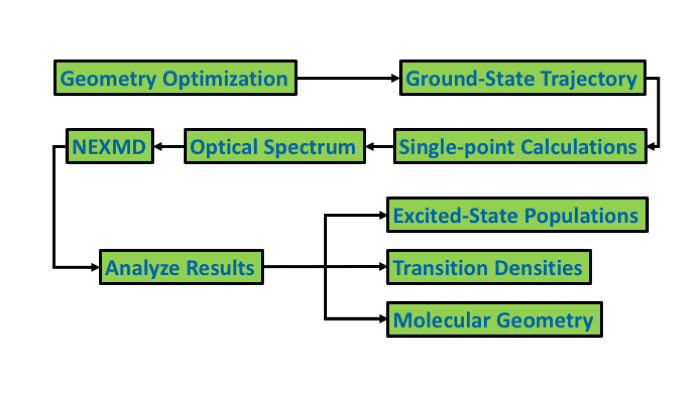
\includegraphics[scale=.6]{general_procedure.png}
	\caption{\small A schematic of the general procedure for simulating non-adiabatic dynamics.}
\label{genproc}
\end{figure}

\newpage
\section{The Input File}
 
The contents of the input file for \verb+NEXMD+ can be categorized as follows: geometry optimization, ground-state parameters, excited-state parameters, solvent models, molecular dynamics, initial geometries and excited-state coefficients.  An overview of all input parameters will be mentioned here, which should be sufficient for getting started with \verb+NEXMD+.  The input file will be discussed one section at a time.  The numerical values in square brackets are default parameters.
\\
\\
The following section contains input parameters pertaining to geometry optimization.
\begin{lstlisting}[mathescape=false,escapeinside={(*@}{@*)}]
&qmmm
   !***** Geometry Optimization
   maxcyc=0, ! Number of cycles for geometry optimization [0]
   ntpr=1, ! Print results every ntpr cycles [1]
   grms_tol=1.0d-2, ! Tolerance in eV/A (derivatives) [1.0d-2]
\end{lstlisting}
\begin{itemize}
\item \verb+maxcyc+ sets the maximum number of cycles for geometry optimization.  If the number of cycles reaches \verb+maxcyc+, an error message reads: \verb+Maximum+ \verb+number+ \verb+of+ \verb+iterations+ \verb+reached+ \verb+without+ \verb+convergence+.  Therefore,  to optimize geometry, \verb+maxcyc+ must be set to a sufficiently large number greater than zero.  If the geometry reaches the maximum number of cycles, you must review the situation carefully to determine if the input geometry was appropriate or if \verb+grms_tol+ (shown below) was set too low.  A negative \verb+maxcyc+ is treated as \verb+0+.
\item \verb+ntpr+ sets how often results for geometry optimization are printed to the standard output file.  The output of the iteration is written as \verb+iter+, \verb+energy+ in eV, and \verb+rms+ \verb+gradient+ in eV per \AA.  The latter quantity is explained in \verb+grms_tol+, shown below.
\item \verb+grms_tol+ sets the convergence criteria for geometry optimization.  The units for \verb+grms_tol+ are in eV per \AA, so that a smaller \verb+grms_tol+ is a smaller change in energy per change in bond length (i.e. a tighter convergence criteria).
\end{itemize}

The following section contains input parameters pertaining to the ground-state calculation and its associated outputs.
\begin{lstlisting}[mathescape=false,escapeinside={(*@}{@*)}]
   !***** Ground-State and Output Parameters
   qm_theory='AM1', ! Integral type, check Amber's SQM for more options [AM1]
   scfconv=1.0d-8, ! Ground-state SCF convergence criteria, eV [1.0d-6]
   verbosity=0, ! QM/MM output verbosity (0-minimum, 5-maximum) 
   ! [1 for dynamics and optimization, 5 for others]
   printdipole=2, ! (0) Unrelaxed transitions, (1) Unrelaxed transitions plus 
   ! total molecular, or (2) Unrelaxed/relaxed transitions plus 
   ! total molecular [1 for dynamics and 2 for single-point]
   printbondorders=0, ! (0) No or (1) Yes [0]
   ! *** UNDER DEVELOPMENT, DO NOT USE ***
   density_predict=0, ! (0) None, (1) Reversible MD, 
   ! or (2) XL-BOMD [0] *** ALL ARE UNDER DEVELOPMENT, DO NOT USE ***
   itrmax=300, ! Max SCF iterations for ground state 
   ! (negative to ignore convergence) [300]
\end{lstlisting}
 \begin{itemize}
\item \verb+qm_theory+ sets the semi-empirical model Hamiltonian.  A list of available Hamiltonians can be found in Ref. \cite{amber2017}.  The majority of studies with \verb+NEXMD+ have used Austin Model 1 (AM1).  
\item \verb+scfconv+ sets the convergence criteria for the self-consistent field (SCF) ground-state energy in eV. In other words, the user requests that the ground-state energy be determined to within \verb+scfconv+ eV.
\item \verb+verbosity+ sets the level of printing of QM/MM related outputs.  The outputs of each level can be found in Ref. \cite{amber2017}.  The verbosity should be set to at least \verb+1+ in order to obtain ground-to-excited state oscillator strengths.  This is important for single-point calculations and obtaining an optical spectrum, as described in Subsections \ref{spcalc} and \ref{optspec}, respectively.
\item \verb+printdipole+ sets the printing level for dipole moments.  There are three options to choose from which are: \verb+(0)+, ground-to-excited state transition dipole moments, \verb+(1)+, same as \verb+(0)+ plus the total molecular dipole moment, and \verb+(2)+, same as \verb+(1)+ plus relaxed and unrelaxed difference dipole moments.
\item \verb+itrmax+ sets the maximum number of cycles for the ground-state SCF calculation.  If the number of cycles reaches \verb+itrmax+, the code will stop.  A negative value for \verb+itrmax+ means the ground-state SCF calculation will go through $\left|\verb+itrmax+\right|$ cycles, regardless of whether or not the convergence criteria in \verb+scfconv+ has been met.
\end{itemize}

The following section contains input parameters pertaining to the excited-state calculation.
\begin{lstlisting}[mathescape=false,escapeinside={(*@}{@*)}]
   !***** Excited-State Parameters
   exst_method=1, ! CIS (1) or RPA (2) [1]
   dav_guess=1, ! Restart Davidson from (0) Scratch, (1) Previous, 
   ! or (2) XL-BOMD [1] *** (2) IS UNDER DEVELOPMENT, DO NOT USE ***
   ftol0=1.0d-7, ! Acceptance tolerance (|emin-eold|) [1.0d-5]
   ftol1=1.0d-8, ! Acceptance tolerance for residual norm [1.0d-5] 
   ! *** UNDER DEVELOPMENT, DO NOT USE ***
   dav_maxcyc=200, ! Max cycles for Davidson diagonalization 
   ! (negative to ignore convergence) [100]
   printcharges=0, ! Print (1) or do not print (0) Mulliken charges of QM atoms [0]
   calcxdens=.false., ! Print (.true.) or do not print (.false.) 
   ! excited-to-excited transition dipole moments [.false.]
\end{lstlisting}
\begin{itemize}
\item \verb+exst_method+ sets the approximate excited-state wavefunction, which is used to compute excited-state properties.  There are two options to choose from in \verb+NEXMD+.  The first is the configuration interactions singles (\verb+CIS+) wavefunction and the other is the random phase approximation wavefunction (\verb+RPA+).  The RPA wavefunction is a slight extension of the CIS wavefunction and includes more electron correlation effects.  Therefore, it is common for RPA to be more computationally demanding than CIS.  The CIS wavefunction is stable and has been used for the majority of studies with \verb+NEXMD+.
\item \verb+dav_guess+ sets the initial guess for the Davidson algorithm.  The Davidson algorithm is used to calculate excited-state eigenvalues and eigenvectors.  One option is to start Davidson from \verb+scratch+.  However, this option may increase computation time.  Another option is start Davidson from results of the \verb+previous+ calculation.  The latter option should be used for realistic simulations.
\item \verb+ftol0+ sets the convergence criteria on excited-state energies.  In other words, the user requests that excited-state energies be determined to within \verb+ftol0+ eV.
\item \verb+dav_maxcyc+ sets the maximum number of cycles for the Davidson algorithm.  If the number of cycles exceeds \verb+dav_maxcyc+, an error message will read: \verb+Number+ \verb+of+ \verb+Davidson+ \verb+iterations+ \verb+exceeded,+ \verb+exiting.+  A negative value for \verb+dav_maxcyc+ means the excited-state calculation will go through $\left|\verb+dav_maxcyc+\right|$ cycles, regardless of whether or not the convergence criteria in \verb+ftol0+ has been met.
\item \verb+printcharges+ sets whether or not to print Mulliken charges of QM atoms to the standard output file.
\item \verb+calcxdens+ sets whether or not to print excited-to-excited transition dipole moments.  This option can only be set to \verb+true+ during single-point calculations.  An error will occur if \verb+calcxdens+ is set to \verb+true+ during dynamics.  A file called \verb+muab.out+ will be generated if \verb+calcxdens=.true.+, which contains excited-to-excited transition dipoles in arbitrary units.  The number of excited states included in \verb+muab.out+ depends on the number of excited states being propagated, which is controlled by \verb+n_exc_states_propagate+, located in an upcoming section of the input file.
\end{itemize}

The following section contains input parameters pertaining to solvent models and external electric fields.
\begin{lstlisting}[mathescape=false,escapeinside={(*@}{@*)}]
   !***** Solvent Models and External Electric Fields
   solvent_model=0, ! (0) None, (1) Linear response, (2) Vertical excitation, 
   ! or (3) State-specific  [0]
   potential_type=1, ! (1) COSMO or (2) Onsager [1]
   onsager_radius=2, ! Onsager radius, A (system dependent) [2]
   ceps=10, ! Dielectric constant, unitless [10]
   linmixparam=1 ! Linear mixing parameter for vertical excitation 
   ! or state-specific SCF calculation [1]
   cosmo_scf_ftol=1.0d-5, ! Vertical excitation or state-specific 
   ! SCF tolerance, eV [1.0d-5]
   doZ=.false. ! Use relaxed (.true.) or unrelaxed (.false) density for 
   ! vertical excitation or state-specific COSMO or Onsager [.false.]
   index_of_refraction=100, ! Dielectric constant for linear response 
   ! solvent in excited state, unitless [100] *** UNDER DEVELOPMENT, DO NOT USE ***
   EF=0, ! (0) None or (1) Electric field in ground and excited state [0]
   Ex=0, ! Electric field vector X, eV/A [0]
   Ey=0, ! Electric field vector Y, eV/A [0]
   Ez=0, ! Electric field vector Z, eV/A [0] 
&endqmmm
\end{lstlisting}
\begin{itemize}
\item \verb+solvent_model+ sets the solvent model.  A description of the models can be found in Refs. \cite{bjorgaard2015solvent1,bjorgaard2015solvent2}.
\item \verb+potential_type+ sets the potential of the solvent model.  The Onsager model assumes that the solute is placed in a spherical cavity inside the solvent. The latter is described as a homogeneous, polarizable medium of constant dielectric constant given by \verb+ceps+. The solute dipole moment induces a dipole moment of opposite direction in the surrounding medium. Polarization of the medium in turn polarizes the charge distribution in the solvent. Treating this mutual polarization in a self-consistent manner leads to the Onsager reaction field model. COSMO (Conductor-like Screening Model) generalizes the Onsager potential where the cavity surface is defined by the shape of the solute.  COSMO is a more complete description of the electrostatic interactions.
\item \verb+onsager_radius+ defines the radius of the spherical cavity for the Onsager reaction field model.  
\item \verb+ceps+ sets the dielectric constant of the solvent.  A list of solvents and their dielectric constants can be found in Ref. \cite{haynes2014crc}.  Be sure to reference Ref. \cite{haynes2014crc}.
\item \verb+linmixparam+ sets the degree to which the last two SCF iterations are mixed.  The mixed solution is used as an input for the following SCF iteration.  The goal of introducing \verb+linmixparam+ is to significantly reduce the high cost of finding the SCF solution by inputting a solvent potential into the current iteration that is extrapolated from previous iterations.  See Refs. \cite{bjorgaard2015solvent1,bjorgaard2015solvent2} for more information.
\item \verb+cosmo_scf_ftol+ sets the convergence criteria of the vertical excitation or state-specific solvent model SCF calculation.  In other words, the user requests that the energy be determined to within \verb+cosmo_scf_ftol+ eV.  The \verb+cosmo_scf_ftol+ flag sets the tolerance for both the Onsager and COSMO potentials.
\item \verb+EF+ sets whether or not there is an external electric field applied to the system.
\item \verb+Ex+, \verb+Ey+, \verb+Ez+ sets the magnitude and direction of the external electric field in the $x$, $y$, and $z$ axes, respectively.  The user must also set \verb+EF+ to \verb+1+ if an external electric field is desired in the simulation.
\end{itemize}

\textit{General Note}: The default tolerances within the section enclosed by \verb+&qmmm+ and \verb+&endqmmm+ are within accepted levels of convergence.  However, these values may be increased depending on the size of the system or time of simulation.
\\
\\
The following section contains general input parameters pertaining to molecular dynamics.
\begin{lstlisting}[mathescape=false,escapeinside={(*@}{@*)}]
&moldyn
   !***** General Parameters
   natoms=12, ! Number of atoms 
   ! (must be equal to the number of atoms in system)
   rnd_seed=19345, ! Seed for the random number generator
   bo_dynamics_flag=0, ! (0) Non-BO or (1) BO [1]
   exc_state_init=6, ! Initial excited state (0 - ground state) [0]
   n_exc_states_propagate=8, ! Number of excited states [0]
\end{lstlisting}
\begin{itemize}
\item \verb+natoms+ sets the number of atoms in the system being studied.  This number is important for memory allocation and must be equal to or greater than the number of atoms in the system.
\item \verb+rnd_seed+ sets the seed for the random number generator.  For each \verb+rnd_seed+, there is a well-defined sequence of random numbers.  For non-adiabatic ensemble simulations, \verb+rnd_seed+ must be different from one trajectory to another.  This ensures the stochastic nature of the simulation, which is important for both the nuclear Langevin dynamics (i.e. coupling of the system to a heat bath) and the surface hopping algorithm,\cite{tully1990molecular} which governs electronic transitions between electronic states (i.e. non-adiabatic dynamics).  The details of how \verb+rnd_seed+ is chosen for non-adiabatic dynamics will be discussed in Subsection \ref{nexmd}. 
\item \verb+bo_dynamics+ sets whether the dynamics is non-Born--Oppenheimer (non-adiabatic) or Born--Oppenheimer (adiabatic).  If the simulation is non-adiabatic, this typically means the user is running an ensemble of trajectories.  This may also be the case for an adiabatic simulation, depending on the study.
\item \verb+exc_state_init+ sets the initial excited-state of the system.  For a non-adiabatic ensemble simulation, a distribution of initial excited-states is needed to model a photo-excited wavepacket of different nuclear geometries.  Therefore, \verb+exc_state_init+ may be different from one trajectory to another.  The details of how \verb+exc_state_init+ is chosen for non-adiabatic dynamics will be discussed in Subsection \ref{nexmd}. 
\item \verb+n_exc_states_propagate+ sets the total number of excited-states to be propagated in the dynamics.  The user must be careful not to include unnecessary higher-energy states if it is unlikely for the system to access those states, as this may greatly increase computation time.  The number of excited-states to include in the simulation is determined by the electronic structure and optical spectrum of the system, which will be discussed in Subsections \ref{spcalc} and \ref{optspec}.
\end{itemize}

The following section contains more inputs for molecular dynamics.
\begin{lstlisting}[mathescape=false,escapeinside={(*@}{@*)}]
   !***** Dynamics Parameters
   time_init=0.0, ! Initial time, fs [0.0]
   time_step=0.1, ! Time step, fs [0.1]
   n_class_steps=10000, ! Number of classical steps [1]
   n_quant_steps=4, ! Number of quantum steps for each classical step [4]
   moldyn_deriv_flag=1, ! (0) None, (1) Analytical, or (2) Numerical [1]
   num_deriv_step=1.0d-3, ! Displacement for numerical derivatives, A [1.0d-3]
   rk_tolerance=1.0d-7, ! Tolerance for the Runge-Kutta propagator [1.0d-7]
\end{lstlisting}
\begin{itemize}
\item \verb+time_init+ sets the initial time of the trajectory.  If the trajectory has not yet begun, then this number is set 0.0 fs.  However, it is common for a trajectory to be restarted from where it left off.  In these cases, the initial time depends on when the previous simulation has ended.  Restart input files will be discussed in Section \ref{restart}.
\item \verb+time_step+ sets the classical time-step of the trajectory.  This is the time-step at which nuclear degrees of freedom are integrated.
\item \verb+n_class_steps+ sets the total number of classical time-steps in the trajectory.  An error message will read: \verb+You+ \verb+must+ \verb+run+ \verb+dynamics+ \verb+(n_class_steps > 0)+ \verb+or+ \verb+geometry+ \verb+optimization+ \verb+(maxcyc > 0).+ \verb+Running+ \verb+both+ \verb+simultaneously+ \verb+is+ \verb+not+ \verb+possible.+
\item \verb+n_quant_steps+ sets the number of quantum steps per classical step.  The nuclear degrees of freedom are integrated with the Velocity Verlet (VV) algorithm, while the electronic degrees of freedom (i.e. the quantum coefficients) are integrated with the Runge-Kutta (RK) algorithm.  The nuclear dynamics are more computationally stable than the quantum coefficients.  The VV algorithm, while less computationally demanding than RK, is sufficient for nuclear dynamics.  Quantum coefficients are more susceptible to computational instabilities and require a more rigorous method for integrating their equations of motion (i.e. the Schr\"{o}dinger equation).
\item \verb+moldyn_deriv_flag+ sets how gradients are calculated.  The options here are numerical or analytical.  Generally, analytical derivatives should be used because they are more computationally stable and less computationally expensive than numerical derivatives.
\item \verb+num_deriv_step+ sets the derivative step-size in units of angstroms (\AA) when the \verb+moldyn_deriv_flag+ is set to \verb+numerical+.
\item \verb+rk_tolerance+ sets the convergence criteria on the quantum coefficients in arbitrary units.  The smaller the \verb+rk_tolerance+, the tighter the convergence criteria.  The user should be careful not to set this quantity too low, as RK may not be able to handle very low tolerance levels.  In these cases, the output file will show an error message that reads, \verb+RK tolerance may be too low+.  The \verb+rk_tolerance+ should be increased and trajectories should be restarted from 0.0 fs.
\end{itemize}

The following section contains input parameters pertaining to non-adiabatic dynamics.
\begin{lstlisting}[mathescape=false,escapeinside={(*@}{@*)}]
   !***** Non-Adiabatic Parameters
   decoher_type=2, ! Type of decoherence: Reinitialize (0) Never, 
   ! (1) At successful hops, (2) At successful plus frustrated hops... 
   ! (3) Persico/Granucci, or (4) Truhlar [2]
   ! *** (3) AND (4) ARE UNDER DEVELOPMENT, DO NOT USE ***
   decoher_e0=0.0, ! Decoherence parameter E0, Hartrees [0.1]
   ! (only for decoher_type = 3 or 4) *** UNDER DEVELOPMENT, DO NOT USE ***
   decoher_c=0.0, ! Decoherence parameter C, unitless [0.1]
   ! (only for decoher_type = 3 or 4) *** UNDER DEVELOPMENT, DO NOT USE ***
   dotrivial=1, ! Do unavoided (trivial) crossing routine (1) or not (0) [1]
   quant_step_reduction_factor=2.5d-2, ! Quantum step reduction factor [2.5d-2]
\end{lstlisting}
\begin{itemize}
\item \verb+decoher_type+ sets the method for decoherence.  The surface hopping method treats nuclear degrees of freedom classically and electronic degrees of freedom quantum mechanically.  Due to the classical treatment of nuclei, there is an overcoherence between quantum states.  In realistic simulations, there should always be some form of decoherence.  Method \verb+0+ does not introduce any form of decoherence and should only be used for code testing or benchmarking purposes.  By reinitializing the quantum coefficients after hops, this introduces a form of decoherence that is instantaneous.  Method \verb+1+ collapses the wavefunction at all successful hops, whereas \verb+2+ collapses the wavefunction at all successful plus frustrated hops.  Frustrated hops are those that were unable to satisfy energy conservation and were rejected.  The methods defined by \verb+3+ and \verb+4+ are categorized as energy-based decoherence corrections, where coefficients are rescaled at classical steps, such that the coherence between two states decays as a function of their energy gap (i.e. a larger energy gap means faster decoherence).  It has been shown that the simple collapse method is sufficient for introducing decoherence.\cite{nelson2013nonadiabatic}   In general, method \verb+2+ should be used for realistic simulations.
\item \verb+decoher_e0+ sets the value of $E_{0}$ in units of Hartrees in the following expression for the decoherence time,
\begin{equation}
\label{decrate}
\tau_{\beta\alpha}=\frac{\hbar}{\left|E_{\beta}\left(t\right)-E_{\alpha}\left(t\right)\right|}\left(C+\frac{E_{0}}{\left({\bf{P}}\cdot\hat{d}_{\beta\alpha}\right)^{2}/2\mu}\right)\,,
\end{equation}
where ${\bf{P}}\cdot\hat{d}_{\beta\alpha}$ is momentum in the direction of non-adiabatic coupling, $E_{i}\left(t\right)$ is the energy of the PES associated to state $\ket{i}$, and $\mu$ is the reduced mass.  In Grannuci's formalism,\cite{granucci2010including,granucci2007critical} the kinetic energy term, $\left({\bf{P}}\cdot\hat{d}_{\beta\alpha}\right)^{2}/2\mu$, is replaced by the \textit{total} kinetic energy, which reduces computational cost since non-adiabatic coupling vector can be ignored.  Truhlar's formalism can be found in Refs. \cite{zhu2004coherent,hack2001natural}.
\item \verb+decoher_c+ sets the value of the unitless parameter, $C$, in Eq. (\ref{decrate}).
\item \verb+dotrivial+ sets whether or not to reduce the time-step in the vicinity of trivial crossings.  See description under \verb+quant_step_reduction_factor+ for more details.  Trivial crossings are identified by the method described in Ref. \cite{fernandez2012identification}.
\item \verb+quant_step_reduction_factor+ sets how much to reduce the quantum step in the vicinity of an unavoided or trivial crossing.  At trivial crossings, the energy gap between the adjacent states is vanishingly small.  The coupling between these states is essentially localized to the spatial {\it{point}} at which they are degenerate.  Therefore, in order to resolve the non-adiabatic coupling between these states and determine whether or not an electronic transition occurs, the time-step must be reduced.  It is defined as \verb+quant_step_reduction_factor+ $\times$ \verb+quant_time_step+, where \verb+quant_time_step+ is determined by \verb+time_step+ and \verb+n_quant_steps+.
\end{itemize}

The following section contains input parameters pertaining to the thermostat.

\begin{lstlisting}[mathescape=false,escapeinside={(*@}{@*)}]
   !***** Thermostat Parameters
   therm_type=1, ! Thermostat type: (0) Newtonian, (1) Langevin, 
   ! or (2) Berendsen [1] *** (2) IS UNDER DEVELOPMENT, DO NOT USE ***
   therm_temperature=300, ! Thermostat temperature, K [300]
   therm_friction=20, ! Thermostat friction coefficient, 1/ps [20]
   berendsen_relax_const=0.4, ! Bath relaxation constant for Berendsen 
   ! thermostat, ps [0.4] *** UNDER DEVELOPMENT, DO NOT USE ***
   heating=0, ! Equilibrated (0) or heating (1) [0]
   ! *** UNDER DEVELOPMENT, DO NOT USE ***
   heating_steps_per_degree=100, ! Number of steps per degree 
   ! *** UNDER DEVELOPMENT, DO NOT USE ***
   ! during heating [100] *** UNDER DEVELOPMENT, DO NOT USE ***
\end{lstlisting}
\begin{itemize}
\item \verb+therm_type+ sets the type of thermostat to be used in the simulation.  This determines the equation of motion governing nuclear dynamics.  There are three options for this input, one of which is \verb+Newtonian+.  This is the same as introducing no thermostat, which should only be used for code testing or benchmarking purposes.  The other two options are \verb+Langevin+ and \verb+Berendsen+.  For the latter, velocities are rescaled to attain the user-defined temperature.  This suppresses thermal fluctuations, which is not consistent with the canonical ensemble.  The Langevin equation of motion is a stochastic differential equation that introduces terms for viscosity and a Gaussian random force that controls temperature in such a way that obeys the canonical ensemble.  In realistic simulations, the thermostat should be set to \verb+Langevin+.
\item \verb+therm_temperature+ sets the temperature of the thermostat in units of Kelvin (K).
\item \verb+therm_friction+ sets the friction parameter for the Langevin thermostat in units of inverse picoseconds $\left(\text{ps}^{-1}\right)$.  This input generally depends on the viscosity of the solvent that is being modeled, however, in most cases, the default parameter should be used.
\item \verb+berendsen_relax_const+ sets the relaxation time constant of the Berendsen thermostat.  The velocities of the nuclei in the system are rescaled at a rate given by inverse \verb+berendsen_relax_const+ in order to reach thermal equilibrium at the user-defined temperature in \verb+therm_temperature+.
\end{itemize}

The following section contains input parameters pertaining to output data.
\begin{lstlisting}[mathescape=false,escapeinside={(*@}{@*)}]
   !***** Output & Log Parameters
   verbosity=2, ! NEXMD output verbosity (0-minimum, 3-maximum)
   ! [2 for dynamics, 3 for optimization and single-point]
   out_data_steps=1, ! Number of steps to write data [1]
   out_coords_steps=10, ! Number of steps to write the restart file [10]
   out_data_cube=0, ! Write (1) or do not write (0) view files to generate cubes [0]
   out_count_init=0, ! Initial count for view files [0]
&endmoldyn
\end{lstlisting}
\begin{itemize}
\item \verb+verbosity+ sets the level of printing of NEXMD related outputs.
\item \verb+out_data_steps+ sets number of steps to write data.  For example, if \verb+time_step=0.1+ and \verb+out_data_steps=2+, data will be written to output files every 0.2 fs.
\item \verb+out_coords_steps+ sets the number of steps to write coordinates, velocities, and quantum coefficients.  The output files for these quantities are in \verb+coords.xyz+, \verb+velocity.xyz+, and \verb+coefficient.out+, respectively.  The rate at which these data are written to the output files also depends on \verb+out_data_steps+.  For example, if \verb+time_step=0.1+, \verb+out_data_steps=2+, and \verb+out_coords_steps=2+, these data will be written every 0.4 fs.  In general, coordinates, velocities, and quantum coefficients are written to their respective output files every \verb+time_step+ $\times$ \verb+out_data_steps+ $\times$ \verb+out_coords_steps+ fs.
\item \verb+out_data_cube+ sets whether or not to generate \verb+.DATA+ files.  These files are later used to generate cube files.  If \verb+out_data_cube+ is set to \verb+1+, \verb+.DATA+ files are generated for every excited state and for every time step.  For example, the file \verb+view0003-0007.DATA+ refers to the $3^{\text{rd}}$ time step and $7^{\text{th}}$ excited state.
\item \verb+out_count_init+ sets the initial time step of the \verb+.DATA+ files.  At the beginning of a trajectory, \verb+out_count_init+ should be set to \verb+0+.  During generation of restart input files, \verb+out_count_init+ will be changed accordingly.
\end{itemize}

The following section contains input parameters pertaining to the coordinates and velocities of the atoms that constitute the molecule being studied, as well as its excited-state coefficients.
\begin{lstlisting}[mathescape=false,escapeinside={(*@}{@*)}]
&coord
  6       -7.9798271101       0.6776918081      -0.0532285388
  6       -7.0849928010       1.7602597759       0.0294961792
  6       -5.7058415294       1.5490364812       0.0312760931
  6       -5.2231419594       0.2195333448      -0.0446043010
  6       -6.1050960756      -0.8685564920       0.0220869421
  6       -7.5344099241      -0.6444487634       0.0248126135
  1       -9.0268081830       0.8587716724      -0.0794794940
  1       -7.4774606514       2.7566353436       0.1635393862
  1       -5.0939335779       2.4479885163       0.1481876938
  1       -4.1292016456       0.0999373674      -0.1580811639
  1       -5.6916991654      -1.8878557992       0.1151090966
  1       -8.2838388636      -1.4313798704       0.1051927200
&endcoord

&veloc
     3.3718248255    -5.6032885851    -1.1970845430
     2.5106648755     2.0978837936    -1.0696411897
    -5.9135180273    -3.7505826950     1.1689299883
     7.7194332369     4.8702351843     0.6576546539
    -7.1851218597    -2.0113572464    -0.6329683366
    -1.7276579899     0.3919019235    -0.0257452789
   -17.0279163131     9.9875659542     5.3513734186
    -4.7222747943    18.9640275032    11.9601977632
    10.9539809532    17.0164104392    -9.7113209726
    25.7548696749     2.2116651958    -0.5444198125
   -16.5303708308    -2.3313274630    -3.2147489925
    16.2776787026     2.2582071549     9.3572624705
&endveloc

&coeff
  0.00  0.00
  0.00  0.00
  0.00  0.00
  0.00  0.00
  0.00  0.00
  1.00  0.00
  0.00  0.00
  0.00  0.00
&endcoeff
\end{lstlisting}
\begin{itemize}
\item Between \verb+&coord+ and \verb+&endcoord+ are coordinates of the atoms in angstroms (\AA).  The first column identifies each atom with its atomic number.  The following three columns are the $x$, $y$, and $z$ coordinates, respectively.  The coordinates shown above are those of a benzene molecule.
\item Between \verb+&veloc+ and \verb+&endveloc+ are three columns showing velocities of each atom along the $x$, $y$, and $z$ axes, respectively.  The units of velocity are \AA/fs. 
\item Between \verb+&coeff+ and \verb+&endcoeff+ are two columns showing the magnitude and phase of the excited-state coefficients, respectively.  The number of rows should be equal to the number of excited states being propagated, \verb+n_exc_states_propagate+.  In this example, eight excited-states are being propagated and the system is initially fully excited in the sixth excited-state. 
\end{itemize}

\newpage
\section{Modeling Photoinduced Dynamics and Preparing Input Files}
\label{prepinputs}

\subsection{Geometry Optimization}
\label{geopt}
The first step before any simulation is to build the chemical system of interest in some molecular visualization tool such as \verb+Jmol+ or \verb+Avogadro+.  Then, the system's ground-state geometry must be determined according to some model quantum-chemistry.  The geometry may be optimized within \verb+NEXMD+ using the available semi-empirical model Hamiltonians.  An example input file is available in Subsection \ref{input_geopt}.  Jobs submissions are discussed in Section \ref{submit}.  Note: It may be necessary to use other levels of theory, such as density functional theory, to obtain an accurate ground-state geometry.  This can be done with electronic structure packages such as \verb+Gaussian+.

\subsection{Ground-State Trajectory}
\label{gstraj}
The molecule is in an absolute ground-state after it is optimized in Subsection \ref{geopt}.  However, in reality, it is in contact with a heated environment, which causes thermal motion due to coupling with vibrational modes.  To some degree, there is no well-defined chemical structure at finite temperature.  The procedure of Subsection \ref{geopt} is still required, however, since the initial geometry cannot be far off from the true ground-state.  The ground-state geometry of the molecule should be sampled from an ensemble of geometries.  This forms the basis of trajectory-based dynamics, where each trajectory starts with coordinates and velocities sampled at different times throughout a ground-state trajectory.  To obtain these geometries, a long ground-state trajectory of the molecule must be calculated, from which coordinates and velocities are outputted at a rate defined in \verb+input.ceon+.  Typically, the ground-state trajectory should be on the order of nanoseconds and the number of coordinates and velocities outputted should be greater than the intended number of non-adiabatic trajectories that are to be computed in Subsection \ref{nexmd}.  The latter depends on a number of factors including the size of the molecule, the number of excited-states being propagated, and the time of the simulation, but in most cases, this number will not exceed one to two thousand.  An example input file is available in Subsection \ref{input_gstraj}.

\subsection{General Outline of getexcited.py}
After completing a long ground-state trajectory and obtaining a good ground-state sampling, the remaining steps shown in Figure \ref{genproc} requires making and manipulating many input and output files in order to simulate and analyze the results from non-adiabatic dynamics.  Many of these steps can be done with \verb+getexcited.py+.  The \verb+getexcited.py+ script is the main script that calls specific functions from the \verb+getexcited_package+.  This package is written in \verb+Python 2.7+ which should be loaded in the terminal with command \verb+module+ \verb+load+ \verb+<version+ \verb+2.7+ \verb+of+ \verb+Python>+.  To get the exact name, type \verb+module+ \verb+avail+ before loading the module.  \textbf{Important}: Before executing \verb+getexcited.py+, it must be opened and the variable \verb+PATHTOPACK+ must be set to the path to where the \verb+getexcited_package+ exists.  The \verb+getexcited_package+ is typically located in a bin folder in your home directory.  A general outline of how one may proceed through steps of modeling non-adiabatic dynamics using \verb+getexcited.py+ is shown in Figure \ref{getexcited_outline}.  Each of these steps will be discussed in this document.  It is worth noting that more steps, not shown in Figure \ref{getexcited_outline} and not discussed in this document, may be necessary depending on the study.
\begin{figure}[t]
	\centering
	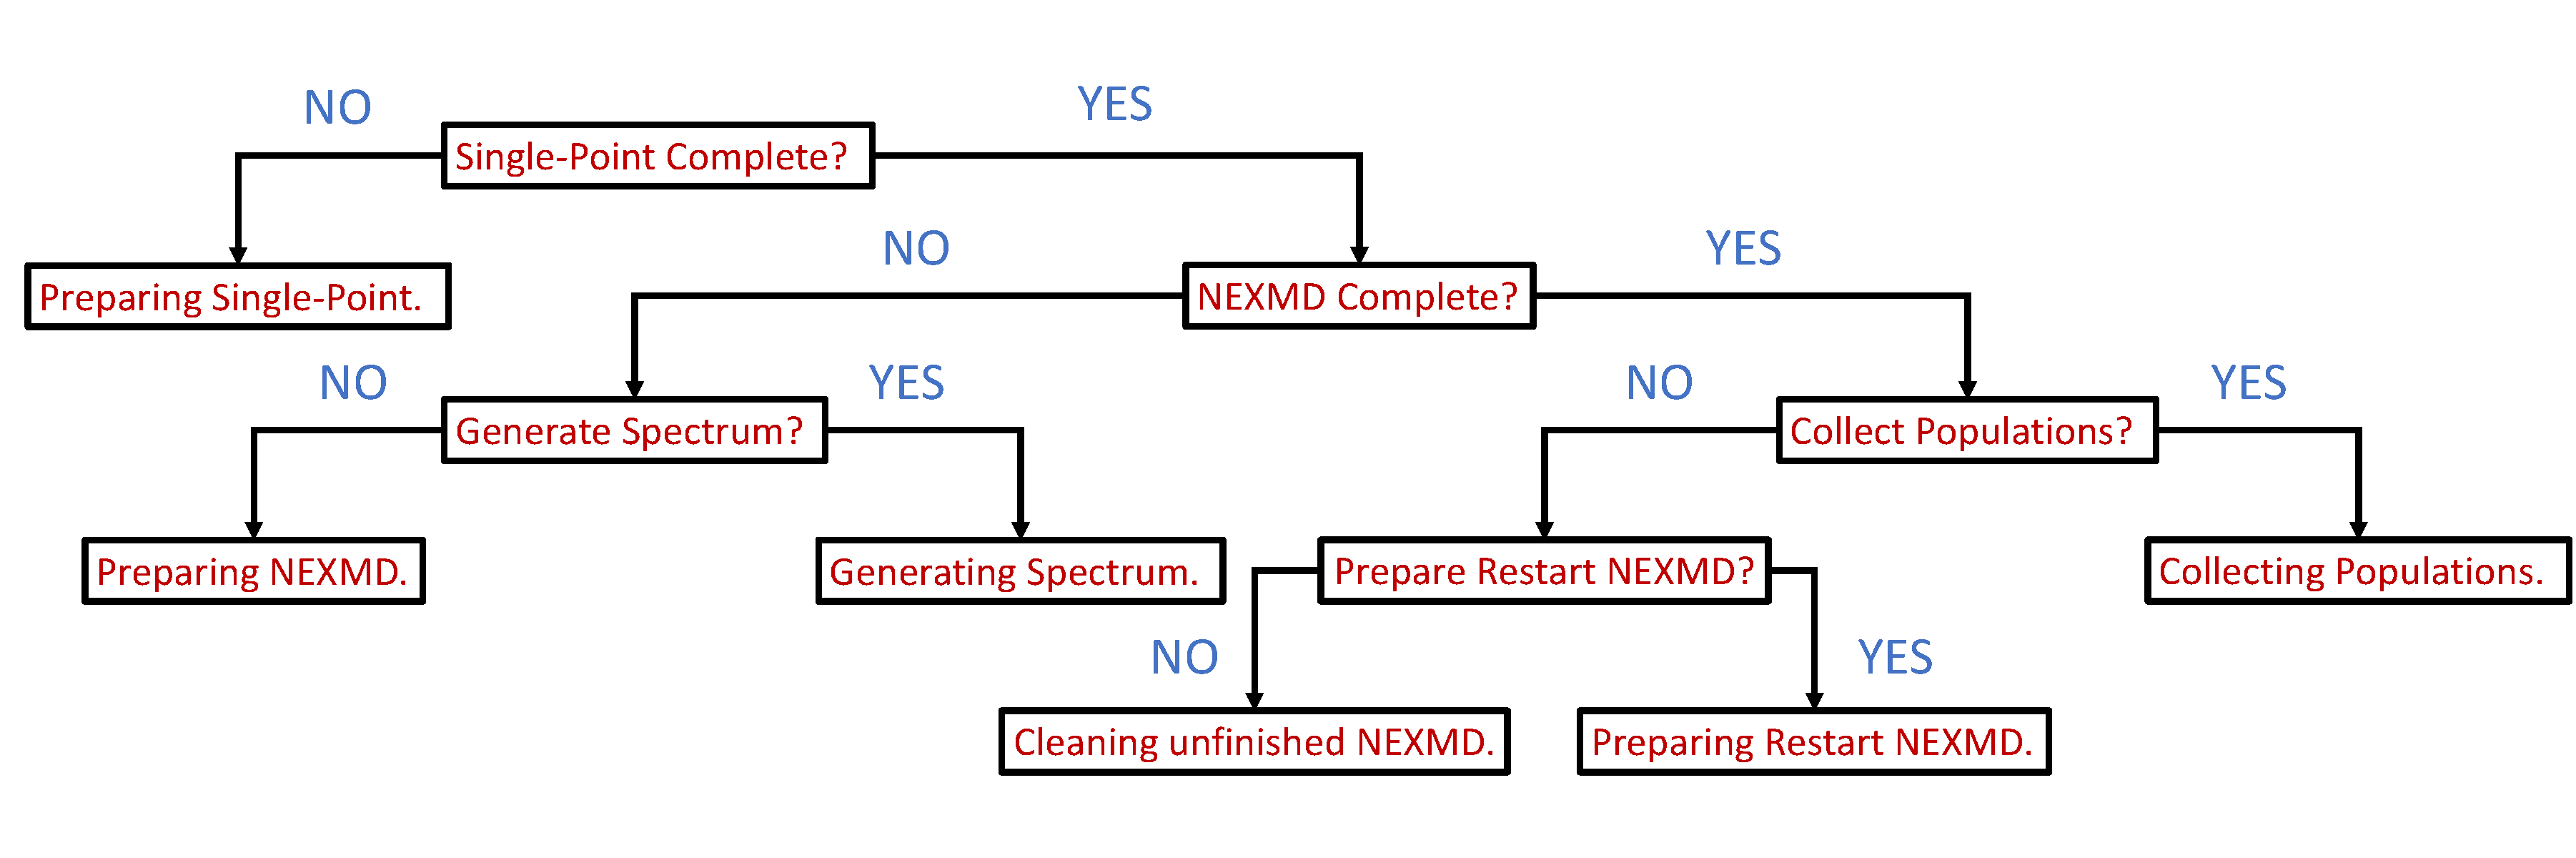
\includegraphics[scale=.27]{getexcited_structure.pdf}
	\caption{\small A schematic in YES or NO question format that proceeds through the different steps of modeling non-adiabatic dynamics.}
	\label{getexcited_outline}
\end{figure}

\subsection{Single-Point Calculations}
\label{spcalc}
Throughout the ground-state trajectory, a set of coordinates and velocities will be written to \verb+coords.xyz+ and \verb+velocity.xyz+.  These files contain snap shots of the system taken throughout the ground-state trajectory at a rate which was specified in Subsection \ref{gstraj}.  After the ground-state trajectory is complete, single-point calculations at these geometries determine the electronic structure and optical spectrum of the system.  It is important to consider many single-point calculations before generating an optical spectrum since the geometry of the system, and therefore electronic structure, changes from one time-step to another due to its interaction with the heat bath.  It is good to plot temperature as a function of time from \verb+temperature.out+ of the ground-state trajectory to know at which time the system has equilibrated.  This happens once the temperature oscillates around the set temperature of the bath (typically 300 K).  {\it{The ground-state sampling should be taken at times after the system has reached thermal equilibrium.}}

To prepare input files for single-point calculations, use \verb+getexcited.py+.  First, create a directory for the single-point calculations (e.g. \verb+singlepoint+).  Second, create an input file with the name \verb+header+ inside \verb+singlepoint+.  In \verb+header+, you must set the parameters which are to be the same for all single-point calculations.  Be sure to set \verb+verbosity+ within \verb+&qmmm+ and \verb+&endqmmm+ to at least \verb+1+ for single-point calculations!  The only varying parameter among the different single-point calculations is geometry.  An example input file is available in Subsection \ref{input_spcalc}.  In place of both nuclear coordinates and velocities, type in the flag, \verb+nucl_coord_veloc+, as shown below.
\begin{lstlisting}[mathescape=false,escapeinside={(*@}{@*)}]
(*@{\vdots\vspace*{3pt}}@*)
&endmoldyn

nucl_coord_veloc

&coeff
(*@{\vdots\vspace*{3pt}}@*)
\end{lstlisting}
The \verb+getexcited.py+ script searches for this flag and generates an input file for each geometry.  Lastly, type \verb+python+ \verb+getexcited.py+.  An example of preparing input files for single-point calculations is shown below.
\newline
\begin{lstlisting}[mathescape=false,escapeinside={(*@}{@*)}]
[sifain@wc-fe1 realistic]$ ls
getexcited.py  gsdynamics  singlepoint
[sifain@wc-fe1 realistic]$ cd singlepoint/
[sifain@wc-fe1 singlepoint]$ ls
header
[sifain@wc-fe1 singlepoint]$ cd ..
[sifain@wc-fe1 realistic]$ python getexcited.py 

Select a task from the following list:

[1] Prepare input files for single-point calculations
[2] Generate an optical spectrum from single-point calculations
[3] Prepare input files for NEXMD
[4] Prepare input files for adiabatic dynamics with geometries from NEXMD
[5] Collect populations from NEXMD
[6] Collect PESs and NACTs from NEXMD
[7] Prepare restart input files for NEXMD
[8] Clean out the directories of NEXMD trajectories that are incomplete
[9] Access options for geometry analysis
[10] Access options for dipole analysis
[11] Access options for transition density analysis
[12] Access options for pump-push-probe spectroscopy (*** UNDER DEVELOPMENT, DO NOT USE ***)
[13] Access code testing tools

Enter the number corresponding to the desired task: 1
Preparing input files for single-point calculations.
Ground-state dynamics directory: gsdynamics
Output directory [e.g. singlepoint]: singlepoint
A total of 1001 coordinates files, ranging from 0.00 to 
100.00 fs in increments of 0.10 fs, were found.
Enter requested range of the ground-state sampling by 
coordinate files and the number of single-point calculations.
Input an array of the form [start, end, number]: [1,1000,500]
You have requested 500 evenly-spaced coordinate files in the range 1 to 1000.
Continue? Answer YES [1] or NO [0]: 1
Number of single-point calculations per NEXMD folder [e.g. 100]: 100
singlepoint/NEXMD1/0001
singlepoint/NEXMD1/0003
singlepoint/NEXMD1/0005
(*@{\vdots\vspace*{3pt}}@*)
singlepoint/NEXMD5/0995
singlepoint/NEXMD5/0997
singlepoint/NEXMD5/0999
[sifain@wc-fe1 realistic]$ cd singlepoint/
[sifain@wc-fe1 singlepoint]$ ls
header  NEXMD1  NEXMD2  NEXMD3  NEXMD4  NEXMD5
\end{lstlisting}

\subsection{Optical Spectrum}
\label{optspec}
It is important to generate an optical spectrum from single-point calculations to determine the energy at which to excite the system.  To do so, use \verb+getexcited.py+, which generates an average spectrum over all geometries (i.e. the sum of all spectra, divided by the number of geometries).  The oscillator strength of each excitation energy is given a Gaussian lineshape with some user-defined width.  This is a Gaussian-shaped Franck-Condon window.  To be more explicit, the optical absorbance of each excitation energy is broadened by a Gaussian lineshape and is weighted by the oscillator strength at that energy,
\begin{equation}
A_{e}^{i}\left(\Omega\right) = f_{ge}^{i}\left(\Omega_{e}\right)\times\frac{1}{\sqrt{2\pi\sigma^{2}}}\,\exp\left[-\frac{\left(\Omega_{e}-\Omega\right)^{2}}{2\sigma^{2}}\right]\,,
\end{equation}
where $A_{e}^{i}$ defines the contribution to the absorbance of the $i^{\text{th}}$ geometry from excited-state $\ket{e}$. The absorbance over all excitation energies becomes
\begin{equation}
A^{i}\left(\Omega\right) = \sum_{e} A_{e}^{i}\left(\Omega\right)\,.
\end{equation}
To obtain the combined optical spectrum, the spectra from all geometries are averaged,
\begin{equation}
A\left(\Omega\right) = \frac{1}{N}\sum_{i} A^{i}\left(\Omega\right)\,.
\end{equation}
where $N$ is the number of geometries.  You may also choose a Lorentzian lineshape of the form
\begin{equation}
A_{e}^{i}\left(\Omega\right) = f_{ge}^{i}\left(\Omega_{e}\right)\times\frac{2}{\Gamma\pi}\frac{1}{1+4\left(\frac{\Omega-\Omega_{ge}}{\Gamma}\right)^{2}}\,,
\end{equation}
where $\Gamma$ is a full width at half maximum (FWHM).

One of three files will be generated in the current working directory if an optical spectrum is requested, \verb+ceo.err+, \verb+ceo_gauss.out+ or \verb+ceo_lorentz.out+.  Shown in \verb+ceo.err+, are directories of single-point calculations that are problematic.  The latter two output files cannot be generated unless all single-point calculations are complete.  There are two types of spectral lineshapes to choose from, Gaussian or Lorentzian.  To obtain the spectrum, type \verb+python getexcited.py+, which generates a set of questions, one of which is spectral broadening of the Franck-Condon window.  An example of generating an optical spectrum is shown below.
\newline
\begin{lstlisting}[mathescape=false,escapeinside={(*@}{@*)}]
[sifain@wc-fe1 realistic]$ ls
getexcited.py  gsdynamics  singlepoint
[sifain@wc-fe1 realistic]$ python getexcited.py 

Select a task from the following list:

[1] Prepare input files for single-point calculations
[2] Generate an optical spectrum from single-point calculations
[3] Prepare input files for NEXMD
[4] Prepare input files for adiabatic dynamics with geometries from NEXMD
[5] Collect populations from NEXMD
[6] Collect PESs and NACTs from NEXMD
[7] Prepare restart input files for NEXMD
[8] Clean out the directories of NEXMD trajectories that are incomplete
[9] Access options for geometry analysis
[10] Access options for dipole analysis
[11] Access options for transition density analysis
[12] Access options for pump-push-probe spectroscopy (*** UNDER DEVELOPMENT, DO NOT USE ***)
[13] Access code testing tools

Enter the number corresponding to the desired task: 2
Generating optical spectrum.
Single-point calculations directory: singlepoint
Checking energies and oscillator strengths. Please wait ...
Spectral lineshape? Answer GAUSSIAN [0] or LORENTZIAN [1]: 0
Spectral broadening (i.e. Gaussian standard deviation) in eV [e.g. 0.15]: 0.15
singlepoint/NEXMD1/1000
singlepoint/NEXMD1/1004
singlepoint/NEXMD1/1008
(*@{\vdots\vspace*{3pt}}@*)
singlepoint/NEXMD5/4988
singlepoint/NEXMD5/4992
singlepoint/NEXMD5/4996
[sifain@wc-fe1 realistic]$ ls
ceo_gauss.out  getexcited.py  gsdynamics  singlepoint
\end{lstlisting}

The columns in \verb+ceo_gauss.out+ or \verb+ceo_lorentz.out+ are the following: energy in eV, followed the spectra of all excited states, respectively.  The last column is the total spectrum, which is the sum of all spectra from columns 1 to $N$, where $N$ is the number of excited states.  Example spectra are shown in Figure \ref{example_spectra}.
\begin{figure*}[h]
        \centering
        \begin{subfigure}[h]{0.475\textwidth}
            \centering
            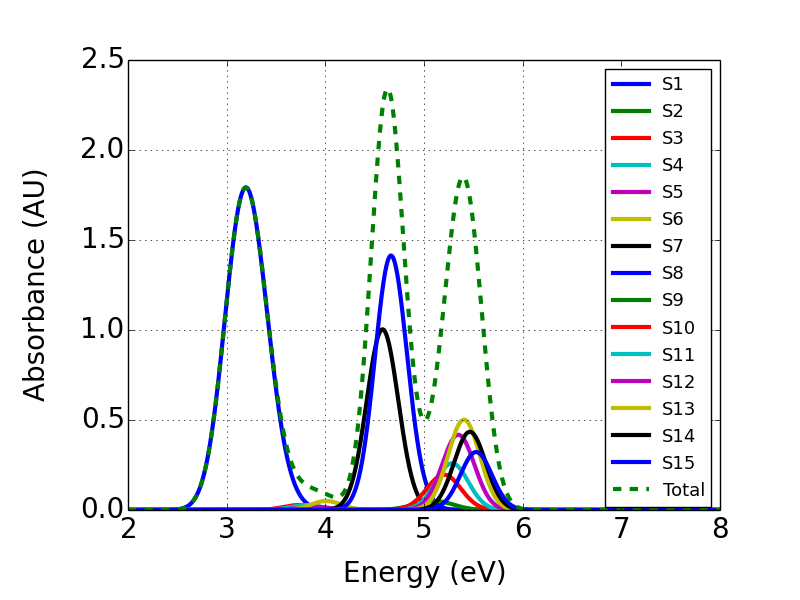
\includegraphics[scale=.4]{spec_gauss.png}
            % 
        \end{subfigure}
	\hspace{3mm}
        \begin{subfigure}[h]{0.475\textwidth}  
            \centering 
            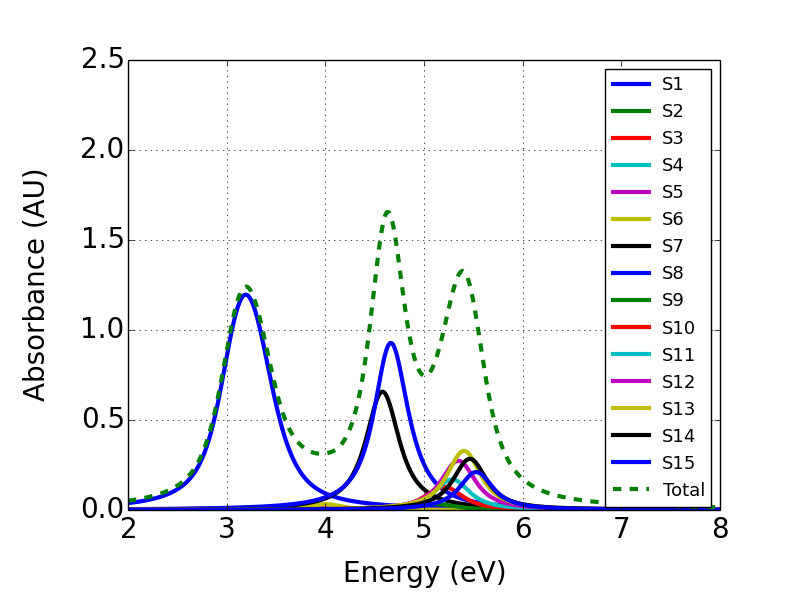
\includegraphics[scale=.4]{spec_lorentz.png}
            %
        \end{subfigure}
	\caption{\small Absorption spectra of a Poly(p-phenylene vinylene) molecule.  Each spectrum is an average over 1000 spectra obtained from 1000 single-point calculations.  The spectra are generated with Gaussian lineshapes (left) and Lorentzian lineshapes (right).}
\label{example_spectra}
\end{figure*}

\subsection{NEXMD}
\label{nexmd}
Input files for NEXMD may be prepared once single-point calculations are complete, and you know at which energy to excite the system.  First, create a directory for NEXMD (e.g. \verb+nexmd+).  Inside \verb+nexmd+, place an input file with the name \verb+header+.  Similar to Subsection \ref{spcalc}, you must set the parameters which are to be the same for all trajectories.  An example input file is available in Subsection \ref{input_nexmd}.  The four parameters that are different among the trajectories are: random seed, initial excited-state, initial nuclear coordinates and velocities, and initial quantum amplitudes and phase.  In place of these parameters, insert their respective flags: \verb+rnd_seed+, \verb+exc_state_init_flag+, \verb+nucl_coord_veloc+, and \verb+quant_amp_phase+.  The \verb+getexcited.py+ script searches for these flags and generates an input file for each initial geometry.

To prepare input files for NEXMD, type \verb+python getexcited.py+.  Among the questions asked is, \verb+New random+ \verb+seeds? Answer YES [1] or NO [0]: +.  By answering \verb+YES+, you are requesting for a new list of random seeds.  By answering \verb+NO+, you are requesting to use a pre-generated list of random seeds.  If you request the former, new random seeds will be used to create input files and the complete list of these random seeds will be generated in the \verb+nexmd+ directory with name \verb+rseedslist+.  If you request the latter, the path to the pre-generated list of random seeds must be supplied in the proceeding question.  The pre-generated list of random seeds must strictly be a list of random seeds with no header or footer, and the number of random seeds must be at least equal to the number of trajectories requested.  The pre-generated list of random seeds option may be important for code testing or benchmarking purposes.  \textit{It is important to keep in mind that different compilers may have different sequences of random numbers for a given random seed.}

You must supply both the excitation energy and spectral broadening of the Franck-Condon window.  The latter quantity should be the same as that supplied in Subsection \ref{optspec}, which was used to generate the optical spectrum.  These two quantities are used to determine \verb+exc_state_init+ and \verb+quant_amp_phase+.  For each initial geometry, excitation energies and oscillator strengths were determined from single-point calculations in Subsection \ref{spcalc}.  In order to determine the initial excited-state of each geometry upon photo-excitation, a Gaussian-shaped Franck-Condon window (centered at the user-defined excitation energy, $\Omega$, with spectral broadening, $\sigma$) is multiplied by each oscillator strength, $f_{eg}$,
\begin{equation}\label{unormp}
P^{\prime}\left(\Omega_{e}\right) = f_{ge}\left(\Omega_{e}\right)\times\frac{1}{\sqrt{2\pi\sigma^{2}}}\,\exp\left[-\frac{\left(\Omega_{e}-\Omega\right)^{2}}{2\sigma^{2}}\right]\,.
\end{equation}
Eq. (\ref{unormp}) is an unnormalized probability of exciting the system at $\Omega_{e}$ with laser energy, $\Omega$.  To determine the probability, $P\left(\Omega_{e}\right)$, Eq. (\ref{unormp}) must be divided by the norm such that,
\begin{equation}
P\left(\Omega_{e}\right) = \frac{P^{\prime}\left(\Omega_{e}\right)}{\sum_{e} P^{\prime}\left({\Omega_{e}}\right)}\,.
\end{equation}
The \verb+getexcited.py+ script then chooses a random number between zero and one and determines \verb+exc_state_init+ for each initial geometry.  In \verb+quant_amp_phase+, the system is set to fully populate \verb+exc_state_init+ (i.e. $c_{e} = 1.0$).  All phase factors are initially set to zero.  An example of preparing input files for NEXMD is shown below.
\begin{lstlisting}[mathescape=false,escapeinside={(*@}{@*)}]
[sifain@wc-fe1 realistic]$ ls
ceo_gauss.out  getexcited.py  gsdynamics  nexmd  singlepoint
[sifain@wc-fe1 realistic]$ cd nexmd/
[sifain@wc-fe1 nexmd]$ ls
header
[sifain@wc-fe1 nexmd]$ cd ..
[sifain@wf-fe1 realistic]$ python getexcited.py 

Select a task from the following list:

[1] Prepare input files for single-point calculations
[2] Generate an optical spectrum from single-point calculations
[3] Prepare input files for NEXMD
[4] Prepare input files for adiabatic dynamics with geometries from NEXMD
[5] Collect populations from NEXMD
[6] Collect PESs and NACTs from NEXMD
[7] Prepare restart input files for NEXMD
[8] Clean out the directories of NEXMD trajectories that are incomplete
[9] Access options for geometry analysis
[10] Access options for dipole analysis
[11] Access options for transition density analysis
[12] Access options for pump-push-probe spectroscopy (*** UNDER DEVELOPMENT, DO NOT USE ***)
[13] Access code testing tools

Enter the number corresponding to the desired task: 3
Preparing input files for NEXMD.
Ground-state dynamics directory: gsdynamics
Single-point calculations directory: singlepoint
Output directory [e.g. nexmd]: nexmd 
A total of 1001 coordinate files, ranging from 0.00 to 
100.00 fs in increments of 0.10 fs, were found.
Note: Only coordinate files used for single-point 
calculations can be used for NEXMD.
How many trajectories for NEXMD? Enter a number no greater than 1000: 1000
Number of trajectories per NEXMD folder: 200
New random seeds? Answer YES [1] or NO [0]: 1
Spectral lineshape? Answer GAUSSIAN [0] or LORENTZIAN [1]: 0
Laser excitation energy in eV: 5.40
Spectral broadening (i.e. Gaussian standard deviation) in eV [e.g. 0.15]: 0.15
nexmd/NEXMD1/0001
nexmd/NEXMD1/0002
nexmd/NEXMD1/0003
(*@{\vdots\vspace*{3pt}}@*)
nexmd/NEXMD5/0998
nexmd/NEXMD5/0999
nexmd/NEXMD5/1000
[sifain@wc-fe1 realistic]$ cd nexmd/
[sifain@wc-fe1 nexmd]$ ls
header  NEXMD1  NEXMD2  NEXMD3  NEXMD4  NEXMD5  rseedslist
\end{lstlisting}

An example of preparing input files for NEXMD with a pre-generated list of random seeds is shown below.
\begin{lstlisting}[mathescape=false,escapeinside={(*@}{@*)}]
[sifain@wc-fe1 realistic]$ ls
ceo_gauss.out  getexcited.py  gsdynamics  nexmd  rseedslist  singlepoint
[sifain@wc-fe1 realistic]$ wc -l rseedslist 
1000 rseedslist
[sifain@wf-fe1 realistic]$ python getexcited.py 

Select a task from the following list:

[1] Prepare input files for single-point calculations
[2] Generate an optical spectrum from single-point calculations
[3] Prepare input files for NEXMD
[4] Prepare input files for adiabatic dynamics with geometries from NEXMD
[5] Collect populations from NEXMD
[6] Collect PESs and NACTs from NEXMD
[7] Prepare restart input files for NEXMD
[8] Clean out the directories of NEXMD trajectories that are incomplete
[9] Access options for geometry analysis
[10] Access options for dipole analysis
[11] Access options for transition density analysis
[12] Access options for pump-push-probe spectroscopy (*** UNDER DEVELOPMENT, DO NOT USE ***)
[13] Access code testing tools

Enter the number corresponding to the desired task: 3
Preparing input files for NEXMD.
Ground-state dynamics directory: gsdynamics
Single-point calculations directory: singlepoint
Output directory [e.g. nexmd]: nexmd 
A total of 1001 coordinate files, ranging from 0.00 to 
100.00 fs in increments of 0.10 fs, were found.
Note: Only coordinate files used for single-point 
calculations can be used for NEXMD.
How many trajectories for NEXMD? Enter a number no greater than 1000: 1000
Number of trajectories per NEXMD folder: 200
New random seeds? Answer YES [1] or NO [0]: 0
Path to random-seeds list: rseedslist
Spectral lineshape? Answer GAUSSIAN [0] or LORENTZIAN [1]: 0
Laser excitation energy in eV: 5.40
Spectral broadening (i.e. Gaussian standard deviation) in eV [e.g. 0.15]: 0.15
nexmd/NEXMD1/0001
nexmd/NEXMD1/0002
nexmd/NEXMD1/0003
(*@{\vdots\vspace*{3pt}}@*)
nexmd/NEXMD1/0998
nexmd/NEXMD1/0999
nexmd/NEXMD1/1000
[sifain@wc-fe1 realistic]$ cd nexmd/
[sifain@wc-fe1 nexmd]$ ls
header  NEXMD1  NEXMD2  NEXMD3  NEXMD4  NEXMD5  rseedslist
\end{lstlisting}

\subsection{Adiabatic Simulation from NEXMD Geometries}
In many cases, the adiabatic dynamics on a low-lying surface can describe important processes, one such example is photo-isomerization observed in a \textit{trans}-to-\textit{cis} conformation change of a molecule.  Upon photo-excitation, the molecule evolves on a high-level surface and then relaxes by exchanging energy to nuclear kinetic energy via transitions to lower-lying excited states.  It is common for the molecule to reach its first excited state and evolve for a considerable amount of time before relaxing to its ground state (possibly in the form of radiative emission).  This is what is known as adiabatic dynamics on the first excited state.  Instead of a non-adiabatic simulation continuing on the first excited-state, it may be necessary to continue dynamics adiabatically.  The advantages of doing so include, reducing computational cost by eliminating the propagation of unnecessary states and increasing the time-step of simulation in order to propagate for longer times.  For this to happen, the final geometries of trajectories in the non-adiabatic simulation must be carried over to the adiabatic simulation.  This can be done with \verb+getexcited.py+.  An example of starting an adiabatic simulation on the first excited-state using geometries from a non-adiabatic simulation is shown below.  \textit{It is important for the molecule to have fully reached the first excited state before beginning adiabatic dynamics.}  See Subsection \ref{relax_rate} to calculate populations.  It is also important to remember to change \verb+exc_state_init+ and \verb+n_exc_states_propagate+ to \verb+1+ in \verb+header+ located in a newly-created directory when adiabatic dynamics on the first excited-state is desired.  The coefficients between \verb+&coeff+ and \verb+&endcoeff+ should be changed to fully populate the first excited state.

\begin{lstlisting}[mathescape=false,escapeinside={(*@}{@*)}]
[sifain@wc-fe1 nexmd_solvent]$ ls
adiabatic_S1   optimize   singlepoint   gsdynamics   getexcited.py   nexmd
[sifain@wc-fe1 nexmd_solvent]$ cd adiabatic_S1/
[sifain@wc-fe1 adiabatic_S1]$ ls
header
[sifain@wc-fe1 adiabatic_S1]$ cd ..
[sifain@wc-fe1 nexmd_solvent]$ python getexcited.py 

Select a task from the following list:

[1] Prepare input files for single-point calculations
[2] Generate an optical spectrum from single-point calculations
[3] Prepare input files for NEXMD
[4] Prepare input files for adiabatic dynamics with geometries from NEXMD
[5] Collect populations from NEXMD
[6] Collect PESs and NACTs from NEXMD
[7] Prepare restart input files for NEXMD
[8] Clean out the directories of NEXMD trajectories that are incomplete
[9] Access options for geometry analysis
[10] Access options for dipole analysis
[11] Access options for transition density analysis
[12] Access options for pump-push-probe spectroscopy (*** UNDER DEVELOPMENT, DO NOT USE ***)
[13] Access code testing tools

Enter the number corresponding to the desired task: 4
Preparing input files for adiabatic dynamics with geometries taken from another simulation.
Ground-state dynamics directory: gsdynamics
NEXMD directory where geometries should be taken from: nexmd
NEXMD directory for new simulation: adiabatic_S1
The coordinates in nexmd began at 0.00 fs and were printed to coords.xyz every 1.00 fs.
New random seeds? Answer YES [1] or NO [0]: 1
At what time, in femtoseconds, should geometries be taken from nexmd? 1000
Finding coordinates and velocities from nexmd.  Please wait ...
adiabatic_S1/NEXMD1/0041
adiabatic_S1/NEXMD1/0100
adiabatic_S1/NEXMD1/0159
(*@{\vdots\vspace*{3pt}}@*)
adiabatic_S1/NEXMD5/29836
adiabatic_S1/NEXMD5/29895
adiabatic_S1/NEXMD5/29954
[sifain@wc-fe1 nexmd_solvent]$ cd adiabatic_S1/
[sifain@wc-fe1 adiabatic_S1]$ ls
header  NEXMD1  NEXMD2  NEXMD3  NEXMD4  NEXMD5  rseedslist
\end{lstlisting}

\newpage
\section{Analyzing Results}

\subsection{Relaxation Rates}
\label{relax_rate}
The relaxation rate of the system after photo-induced excitation is a common quantity of interest.  This can be obtained by fitting excited-state populations as a function of time to some fitting function.  One such example is an exponential function of the form $P\left(t\right)=A-B\exp\left[-k\left(t-t_{0}\right)\right]$, where $A-B$ is the initial population at time $t=t_{0}$, $A$ is the final population as $t\rightarrow\infty$, and $k$ is the relaxation rate.  Other fitting functions may be better-suited depending on how the population evolves.  In any case, you must first collect populations as a function of time from NEXMD simulations.  To do so, use \verb+getexcited.py+.

If collecting populations is requested, two files may be generated in the current working directory, \verb+pop.err+ and \verb+pop.out+.  Shown in \verb+pop.err+, are directories of trajectories that did not complete within the user-defined time.  The last column in \verb+pop.err+ shows the last time-step of the simulation.  In \verb+pop.out+, first column is time in femtoseconds, followed by the average population on each potential energy surface (PES), followed by the sum of all PES populations (i.e. which should be 1.0), followed by the average populations from quantum coefficients, followed by the sum of quantum populations (i.e. which should also be 1.0).  \verb+Completed+ \verb+trajectories+ are those that finish within the user-defined time.  \verb+Excellent+ \verb+trajectories+ are those that finish with the time defined in \verb+header+ located in the NEXMD directory (e.g. \verb+nexmd+).  Unlike Subsection \ref{optspec}, \verb+pop.out+ can be generated even if a set of trajectories did not complete within the user-defined time.  However, it is highly recommended that a sufficient sampling size be obtained before analyzing relaxation rates.  Incomplete trajectories can be restarted from their last time-steps.  This is discussed in Section \ref{restart}.  An example of collecting populations is shown below.
\begin{lstlisting}[mathescape=false,escapeinside={(*@}{@*)}]
[sifain@wc-fe1 realistic]$ python getexcited.py 

Select a task from the following list:

[1] Prepare input files for single-point calculations
[2] Generate an optical spectrum from single-point calculations
[3] Prepare input files for NEXMD
[4] Prepare input files for adiabatic dynamics with geometries from NEXMD
[5] Collect populations from NEXMD
[6] Collect PESs and NACTs from NEXMD
[7] Prepare restart input files for NEXMD
[8] Clean out the directories of NEXMD trajectories that are incomplete
[9] Access options for geometry analysis
[10] Access options for dipole analysis
[11] Access options for transition density analysis
[12] Access options for pump-push-probe spectroscopy (*** UNDER DEVELOPMENT, DO NOT USE ***)
[13] Access code testing tools

Enter the number corresponding to the desired task: 5
Collecting populations.
NEXMD directory: nexmd 
Collect populations up to what time in femtoseconds: 1000
nexmd/NEXMD1/0101 1000.00
nexmd/NEXMD1/0102 1000.00
nexmd/NEXMD1/0103 1000.00
(*@{\vdots\vspace*{3pt}}@*)
nexmd/NEXMD4/0997 1000.00
nexmd/NEXMD4/0999 1000.00
nexmd/NEXMD4/1000 1000.00
Total Trajectories: 0400
Completed Trajectories: 0399
Excellent Trajectories: 0399
One or more trajectories did not finish within 1000.00 femtoseconds, check pop.err.
[sifain@wc-fe1 realistic]$ ls
ceo_gauss.out  getexcited.py  gsdynamics  nexmd  pop.err  pop.out  singlepoint
\end{lstlisting}

Once \verb+pop.out+ is obtained, excited-state populations may be plotted.  Select states may be fit to fitting functions to determine rates.  An example is shown in Figure \ref{pop_fit}.
\begin{figure*}[h]
        \centering
        \begin{subfigure}[h]{0.475\textwidth}
            \centering
            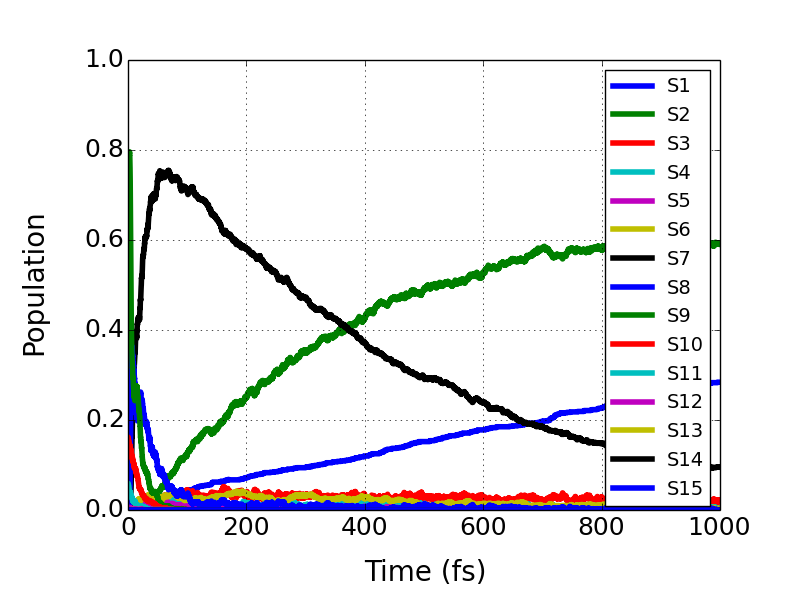
\includegraphics[scale=.4]{pop_hops_allstates.png}
            % 
        \end{subfigure}
	\hspace{3mm}
        \begin{subfigure}[h]{0.475\textwidth}  
            \centering 
            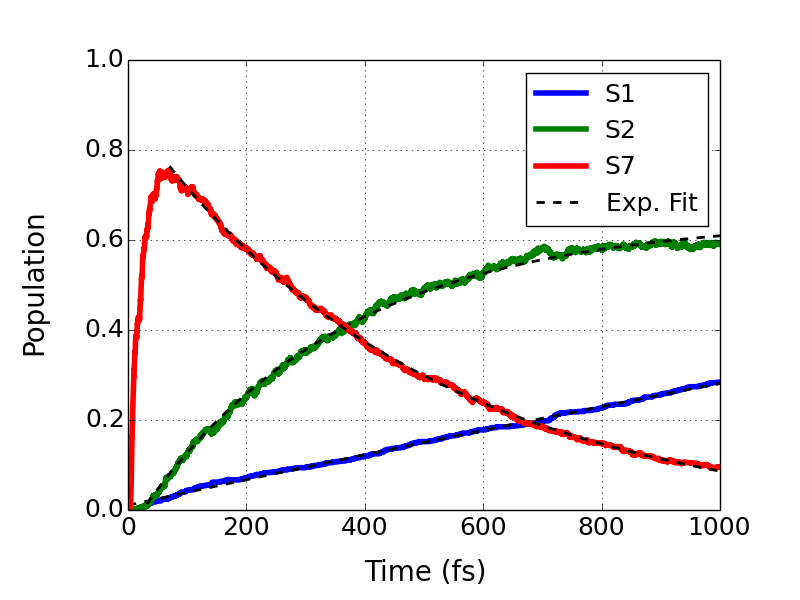
\includegraphics[scale=.4]{pop_hops_expfit.png}
            %
        \end{subfigure}
        \caption{\small Left: Populations of all 15 excited-states from surface hopping in a Poly(p-phenylene vinylene) molecule.  Right: Fitted populations of the states of interest.  In this case, exponential fits were made to S1, S2, and S7.} 
\label{pop_fit}
\end{figure*}

The parameters of the fits are shown below.
\begin{lstlisting}[mathescape=false,escapeinside={(*@}{@*)}]
S1: [A, B, k] = [2.27824e+00, 2.26779e+00, 1.27228e-04]
S2: [A, B, k] = [6.47593e-01, 6.95430e-01, 2.90113e-03]
S7: [A, B, k] = [-3.36844e-02, -7.97627e-01, 2.03588e-03]
\end{lstlisting}

\subsection{PESs and NACTs}
Analyzing excited-state lifetimes may involve explicity looking into the coupling between states, given by non-adiabatic coupling terms (NACTs).  They are of the form $\dot{{\bf{R}}}\cdot {\bf{d}}_{\alpha\beta}$, where $\dot{{\bf{R}}}$ is velocity and ${\bf{d}}_{\alpha\beta}$ is the non-adiabatic coupling vector between states $\ket{\alpha}$ and $\ket{\beta}$.  The latter can be expressed as
\begin{equation}
\label{nacvec}
{\bf{d}}_{\alpha\beta} = \frac{\left<\alpha|\nabla H|\beta\right>}{E_{\beta}-E_{\alpha}}\,,
\end{equation}
where $\nabla H$ is the gradient of the Hamiltonian and $E_{i}$ is the potential energy surface (PES) corresponding to state $\ket{i}$.  Eq. (\ref{nacvec}) shows how non-adiabatic coupling between two states is inversely proportional to the energy gap between those states.  As $|E_{\beta}-E_{\alpha}|$ becomes small, $|{\bf{d}}_{\alpha\beta}|$ becomes large and the system may transition between these excited-states.  The strength of non-adiabatic coupling largely depends on energy gap, making it a useful parameter to analyze.

There are several files that can be generated if collecting NACTs and/or PESs are requested.  You may choose to request PESs and NACTs at all time-steps or only at time-steps where hops occur.  If the latter is requested, two files can be generated, \verb+nact_hop_ensemble.out+ and \verb+pes_hop_ensemble.out+.  In \verb+nact_hop_ensemble.out+, columns from left to right are: directory of trajectory, excited-state at time $t$, excited-state at time $t+\Delta t$, and time in fs.  The remaining columns are NACTs, which are consecutive rows of the upper triangle of the NACT matrix.  For example, for a 2-state system, the indices of these terms would be 11, 12, and 22, respectively.  In \verb+pes_hop_ensemble.out+, the first four columns are the same as those in \verb+nact_hop_ensemble.out+.  The remaining columns are PESs of the ground state followed by all the excited-state PESs in units of eV.  If data at all time-steps are requested, two files can be generated, \verb+nact_raw_ensemble.out+ and \verb+pes_raw_ensemble.out+.  The format of these files are the same as those of \verb+nact_hop_ensemble.out+ and \verb+pes_hop_ensemble.out+, respectively, with the exception that the first column is trajectory directory.  A specific time of collection may be set for cases in which the user is only interested in data up to some time less than the total simulation time.  An example of collecting NACTs and PESs is shown below.
\begin{lstlisting}[mathescape=false,escapeinside={(*@}{@*)}]
[sifain@wc-fe1 realistic]$ ls
ceo_gauss.out  getexcited.py  gsdynamics  nexmd  pop.out  singlepoint
[sifain@wc-fe1 realistic]$ python getexcited.py 

Select a task from the following list:

[1] Prepare input files for single-point calculations
[2] Generate an optical spectrum from single-point calculations
[3] Prepare input files for NEXMD
[4] Prepare input files for adiabatic dynamics with geometries from NEXMD
[5] Collect populations from NEXMD
[6] Collect PESs and NACTs from NEXMD
[7] Prepare restart input files for NEXMD
[8] Clean out the directories of NEXMD trajectories that are incomplete
[9] Access options for geometry analysis
[10] Access options for dipole analysis
[11] Access options for transition density analysis
[12] Access options for pump-push-probe spectroscopy (*** UNDER DEVELOPMENT, DO NOT USE ***)
[13] Access code testing tools

Enter the number corresponding to the desired task: 6
Collecting PESs and NACTs.
NEXMD directory: nexmd
Collect PESs and NACTs up to what time in femtoseconds: 1000
Collect PESs [1], NACTs [2], or BOTH [3]: 3
Collect PESs and NACTs from All TIME-STEPS [1] or HOPS ONLY [2]: 2
nexmd/NEXMD1/1000 1000.00
nexmd/NEXMD1/1004 1000.00
nexmd/NEXMD1/1008 1000.00
(*@{\vdots\vspace*{3pt}}@*)
nexmd/NEXMD5/4988 1000.00
nexmd/NEXMD5/4992 1000.00
nexmd/NEXMD5/4996 1000.00
Total Trajectories: 1000
Completed Trajectories: 1000
Excellent Trajectories: 1000
[sifain@wc-fe1 realistic]$ ls
ceo_gauss.out  getexcited.py  gsdynamics  nact_hop_ensemble.out  nexmd  pes_hop_ensemble.out  pop.out  singlepoint
\end{lstlisting}
An example histogram from the data in \verb+pes_hop_ensemble.out+ is shown in Figure \ref{peshist}.
\begin{figure}[h]
        \centering
        \begin{subfigure}[h]{0.475\textwidth}
            \centering
            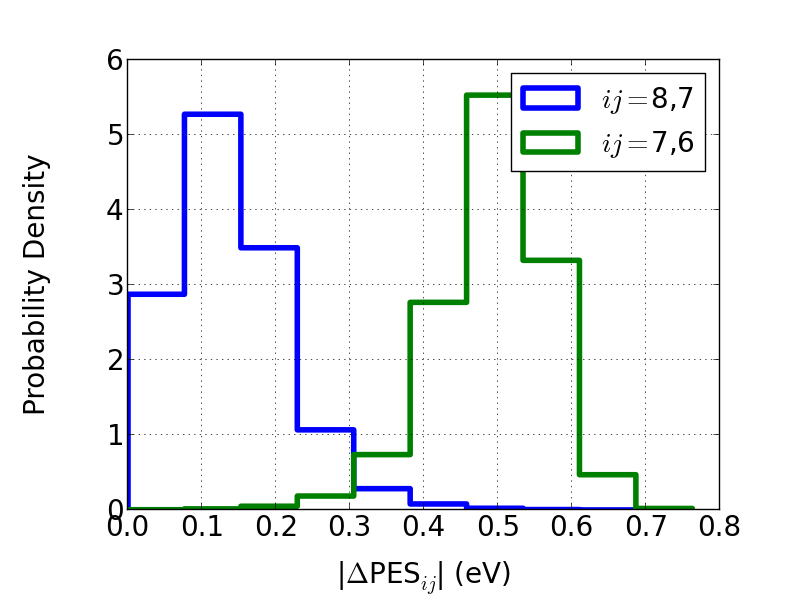
\includegraphics[scale=.4]{pes_hist_all.png}
            % 
        \end{subfigure}
	\hspace{3mm}
        \begin{subfigure}[h]{0.475\textwidth}  
            \centering 
            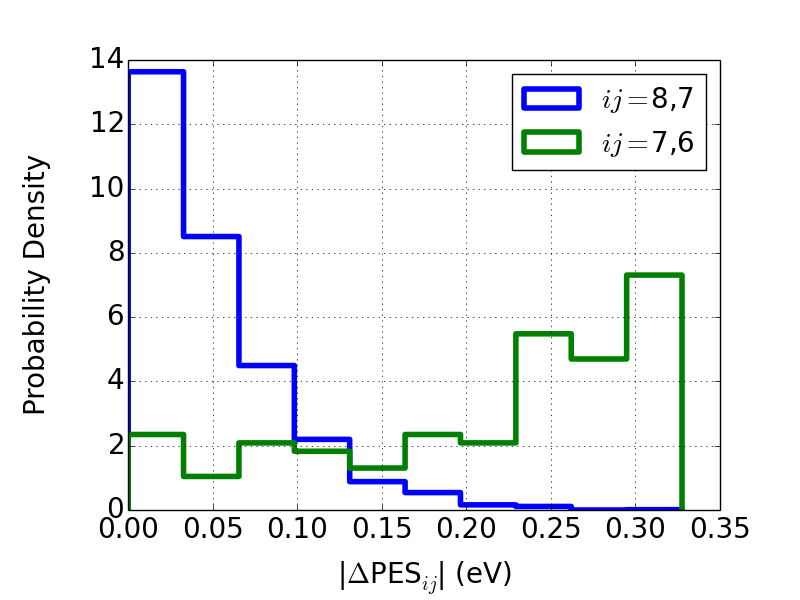
\includegraphics[scale=.4]{pes_hist_hops.png}
            %
        \end{subfigure}
        \caption{\small (Left) Histogrammed data of energy gaps, $|\Delta\text{PES}_{ij}|=|E_{j}-E_{i}|$ for $ij=\{87, 76\}$, at all time-steps in a 1000 trajectory ensemble, where each trajectory is 1.0 ps in length.  (Right) Histogrammed data of the same energy gaps, but only at hops $8\rightarrow7$ and $7\rightarrow6$, respectively.  The number of hops $8\rightarrow7$ and $7\rightarrow6$ are 3044 and 573, respectively.}
\label{peshist}
\end{figure}
In this example, hops from $8\rightarrow7$ and $7\rightarrow6$ as a function of their energy gap are histogrammed.  The number of hops $8\rightarrow7$ is 3044, whereas the number of hops $7\rightarrow6$ is 573.  The energy gap, $|\Delta\text{PES}_{87}|$, is noticeably smaller than $|\Delta\text{PES}_{87}|$, which is likely correlated to the large difference in the number of hops.

\subsection{Geometry Analysis}
There may be conformational changes of the molecule due to photoinduced dynamics.  This can be analyzed as a function of a time.  There are several geometrical quantities that can be calculated with \verb+getexcited.py+, which include dihedrals, bond lengths, and bond length alternations (BLA).  \textit{Dihedral:} The dihedral is calculated from four atoms, where the first three atoms define one plane and the last three atoms define the other plane.  The dihedral is defined as the positive angle between these planes and ranges from 0 to 180 degrees.  \textit{Bond length:} The bond length is calculated using Pythagorean theorem.  \textit{BLA:} BLA is calculated from four atoms giving three consecutive bond lengths, where the first and third have the same bond order and the second has a different bond order.  The BLA is defined as $\left(d_{1}+d_{3}\right)/2 - d_{2}$, where $d_{i}$ is the $i^{\text{th}}$ bond length.  An example of calculating the mean dihedral angle as a function of time over all trajectories is shown below.  The four atoms defining the dihedral are shown below.
\begin{figure}[h]
	\centering 
	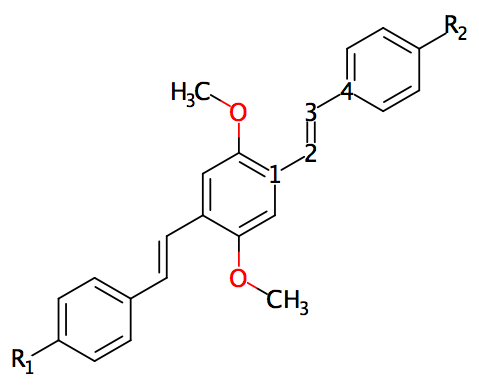
\includegraphics[scale=.50]{asymm_dihedral.png}
\end{figure}

\begin{lstlisting}[mathescape=false,escapeinside={(*@}{@*)}]
[sifain@wc-fe1 realistic]$ ls
getexcited.py  gsdynamics  nexmd  singlepoint
[sifain@wc-fe1 realistic]$ python getexcited.py 

Select a task from the following list:

[1] Prepare input files for single-point calculations
[2] Generate an optical spectrum from single-point calculations
[3] Prepare input files for NEXMD
[4] Prepare input files for adiabatic dynamics with geometries from NEXMD
[5] Collect populations from NEXMD
[6] Collect PESs and NACTs from NEXMD
[7] Prepare restart input files for NEXMD
[8] Clean out the directories of NEXMD trajectories that are incomplete
[9] Access options for geometry analysis
[10] Access options for dipole analysis
[11] Access options for transition density analysis
[12] Access options for pump-push-probe spectroscopy (*** UNDER DEVELOPMENT, DO NOT USE ***)
[13] Access code testing tools

Enter the number corresponding to the desired task: 9

Select a task from the following list:

[1] Calculate a dihedral angle
[2] Calculate a bond length
[3] Calculate a bond length alternation

Enter the number corresponding to the desired task: 1
Calculating a dihedral angle as a function of time.
Calculate a dihedral along one trajectory or an ensemble of trajectories? 
Answer ONE [1] or ENSEMBLE [0]: 0
Ensemble directory [e.g. nexmd]: nexmd_opt
Ouput mean dihedral in time or output dihedrals at all time-steps and trajectories? 
Answer MEAN [0] or ALL [1]: 0
Calculate dihedral up to what time in femtoseconds?
Note that averaged results will only include trajectories that are complete up to this time: 1000
Input the line numbers labeling the coordinates of the four atoms.
Input an array of the form [ .., .., .., .. ]: [1,2,3,4]
nexmd/NEXMD1/1000 1000.00
nexmd/NEXMD1/1004 1000.00
nexmd/NEXMD1/1008 1000.00
(*@{\vdots\vspace*{3pt}}@*)
nexmd/NEXMD5/4988 1000.00
nexmd/NEXMD5/4992 1000.00
nexmd/NEXMD5/4996 1000.00
Total Trajectories: 1000
Completed Trajectories: 1000
Excellent Trajectories: 1000
[sifain@wc-fe1 realistic]$ ls
dihedral.out  getexcited.py  gsdynamics  nexmd  singlepoint
\end{lstlisting}

\newpage
\subsection{Dipole Analysis}
\label{dipanalysis}

The dipole moment of the molecule can be tracked as a function of time throughout its excited state dynamics.  Given the occupied state at a given time-step, the dipole of that state can be extracted from the standard output file.  Note that in order for permanent (or total) dipole data to be available in the standard output file, the user must set \verb+printdipole = 1+ or more.  Dipole analysis can be done on a single trajectory (\verb+permdipole_raw_single.out+) or an ensemble of trajectories.  For the latter, the mean over all trajectories (\verb+permdipole_mean_ensemble.out+) or the raw data over all trajectories and time-steps (\verb+permdipole_raw_ensemble+) may be requested.  In \verb+permdipole_raw_single.out+ and \verb+permdipole_mean_ensemble.out+, columns from left to right are: time (fs) and dipole moment (Debye).  For the latter, there is third column with standard deviation.  Columns in \verb+permdipole_raw_ensemble.out+ are the same as those in \verb+permdipole_raw_single.out+ except that the first column is trajectory directory.   {\textit{Note that this function only works for excited-state dynamics, and that the dipole moment of the ground state is not yet available.}}  An example of calculating the mean dipole as a function of time is shown below.

\begin{lstlisting}[mathescape=false,escapeinside={(*@}{@*)}]
[sifain@wc-fe1 realistic]$ ls
getexcited.py    gsdynamics     nexmd    singlepoint
[sifain@wc-fe1 realistic]$ python getexcited.py 

Select a task from the following list:

[1] Prepare input files for single-point calculations
[2] Generate an optical spectrum from single-point calculations
[3] Prepare input files for NEXMD
[4] Prepare input files for adiabatic dynamics with geometries from NEXMD
[5] Collect populations from NEXMD
[6] Collect PESs and NACTs from NEXMD
[7] Prepare restart input files for NEXMD
[8] Clean out the directories of NEXMD trajectories that are incomplete
[9] Access options for geometry analysis
[10] Access options for dipole analysis
[11] Access options for transition density analysis
[12] Access options for pump-push-probe spectroscopy (*** UNDER DEVELOPMENT, DO NOT USE ***)
[13] Access code testing tools

Enter the number corresponding to the desired task: 10

Select a task from the following list:

[1] Collect excited-state permanent dipole moment

Enter the number corresponding to the desired task: 1
Calculating the permanent dipole moment as a function of time.
Calculate dipole moment along one trajectory or an ensemble of trajectories?
Answer ONE [1] or ENSEMBLE [0]: 0
Ensemble directory [e.g. nexmd]: nexmd/0009
Output mean dipole in time or output dipoles at all time-steps and trajectories?
Answer MEAN [0] or ALL [1]: 0
Calculate dipole up to what time in femtoseconds?
Note that averaged results will only include trajectories that are complete up to this time: 1000
Checking permanent dipole moments and states.  Please wait ...
nexmd/NEXMD1/0041 dipole lines in md.out found
nexmd/NEXMD1/0041 dipoles in md.out extracted
nexmd/NEXMD1/0100 dipole lines in md.out found
nexmd/NEXMD1/0100 dipoles in md.out extracted
(*@{\vdots\vspace*{3pt}}@*)
nexmd/NEXMD5/29895 dipole lines in md.out found
nexmd/NEXMD5/29895 dipoles in md.out extracted
nexmd/NEXMD5/29954 dipole lines in md.out found
nexmd/NEXMD5/29954 dipoles in md.out extracted
nexmd/NEXMD1/0041 1000.00
nexmd/NEXMD1/0100 1000.00
(*@{\vdots\vspace*{3pt}}@*)
nexmd/NEXMD5/29895 1000.00
nexmd/NEXMD5/29954 1000.00
Total Trajectories: 0508
Completed Trajectories: 0508
Excellent Trajectories: 0508
[sifain@wc-fe1 nexmd_solvent]$ ls
getexcited.py    gsdynamics     nexmd    permdipole.out    singlepoint
\end{lstlisting}

\newpage
\subsection{Transition Density Analysis}
The evolution of the electronic wavefunction can be tracked by changes in the spatial localization of the transition density (TD).  Diagonal elements of the TD matrices $\left(\rho^{g\alpha}\right)_{nn}\left(t\right)\equiv\left<\phi_{\alpha}\left(t\right)|c_{n}^{\dagger}c_{n}|\phi_{g}\left(t\right)\right>$ represent changes in the electronic density in an atomic orbital (AO) when undergoing a ground- to excited-state transition, where $c_{n}^{\dagger}$ and $c_{n}$ are creation and annihilation operators, respectively, and $n$ refers to the AO basis function.\cite{wu2006exciton}  The fraction of TD localized on a molecular fragment is the sum of all atomic contributions.\cite{baer2006beyond}  TD analysis describes evolution of the electronic wavefunction without relying on adiabatic state populations, thereby providing a simple way of determining the spatial localization of excitations in time.\cite{fernandez2012identification,fernandez2012shishiodoshi,nelson2013conformational}  

If TD analysis is requested, an input file must be provided which splits the molecule into fragments.   This is accomplished by defining atom numbers according to how they are ordered in a general input file between \verb+&coord+ and \verb+&endcoord+.  The atom numbers are to be written in a user-generated file, where the keyword \verb+break+ is to be inserted wherever a new fragment of the molecule is defined.  An example of which is shown below.
\begin{lstlisting}[mathescape=false,escapeinside={(*@}{@*)}]
1
2
3
4
break
5
6
7
8
\end{lstlisting}

In this example, the molecule contains 8 atoms and is split in half where the first four atoms between \verb+&coord+ and \verb+&endcoord+ define one fragment and the remaining atoms define the other fragment.  TD analysis can be done on a single trajectory (\verb+td_single.out+) or an ensemble of trajectories.  For the latter, the mean over all trajectories (\verb+td_mean_ensemble.out+) or the raw data over all trajectories and time-steps (\verb+td_raw_ensemble+) may be requested.  In \verb+td_single.out+ and \verb+td_mean_ensemble.out+, columns from left to right are: time (fs), followed by the occupations of all fragements in the same order as they were defined in the user-generated fragment file, followed by the sum of all contributions (should be equal to 1.0).  Columns in \verb+td_raw_ensemble.out+ are the same as those in \verb+td_mean_ensemble.out+ except that the first column is trajectory directory.  An example of performing TD analysis is shown below.
\begin{lstlisting}[mathescape=false,escapeinside={(*@}{@*)}]
[sifain@wc-fe1 realistic]$ ls
frag_HH_asymm  getexcited.py  gsdynamics  nexmd  singlepoint
[sifain@wc-fe1 realistic]$ python getexcited.py 

Select a task from the following list:

[1] Prepare input files for single-point calculations
[2] Generate an optical spectrum from single-point calculations
[3] Prepare input files for NEXMD
[4] Prepare input files for adiabatic dynamics with geometries from NEXMD
[5] Collect populations from NEXMD
[6] Collect PESs and NACTs from NEXMD
[7] Prepare restart input files for NEXMD
[8] Clean out the directories of NEXMD trajectories that are incomplete
[9] Access options for geometry analysis
[10] Access options for dipole analysis
[11] Access options for transition density analysis
[12] Access options for pump-push-probe spectroscopy (*** UNDER DEVELOPMENT, DO NOT USE ***)
[13] Access code testing tools

Enter the number corresponding to the desired task: 11

Select a task from the following list:

[1] Analyze occupancy according to diagonal elements of the transition density matrix

Enter the number corresponding to the desired task: 1
Calculating occupation of excitation as a function of time according to transition densities.
Calculate occupation along one trajectory or an ensemble of trajectories?
Answer ONE [1] or ENSEMBLE [0]: 0
Ensemble directory [e.g. nexmd]: nexmd
Output mean occupation in time, at all time-steps and trajectories, 
or up to some user-defined time? Answer MEAN [0], ALL [1], or USER-DEFINED [2]: 0
Directory with an input.ceon file for coordinates, do not include input.ceon in the path: 
nexmd/NEXMD1/0041
Directory with fragment file, include name of file in the path: frag_HH_asymm
Calculate occupation up to what time in femtoseconds?
Note that averaged results will only include trajectories that are 
complete up to this time: 100
nexmd/NEXMD1/0041 1000.00
nexmd/NEXMD1/0100 1000.00
nexmd/NEXMD1/0159 1000.00
(*@{\vdots\vspace*{3pt}}@*)
nexmd/NEXMD5/29836 1000.00
nexmd/NEXMD5/29895 1000.00
nexmd/NEXMD5/29954 1000.00
Total Trajectories: 0508
Completed Trajectories: 0508
Excellent Trajectories: 0508
[sifain@wc-fe1 realistic]$ ls
frag_HH_asymm  getexcited.py  gsdynamics  nexmd  singlepoint  td_mean_ensemble.out
\end{lstlisting}

\newpage
\section{Code Testing Tools}

\subsection{Timings}
CPU times can be obtained from trajectories of an ensemble.  The timing data is divided up among \verb+ground state+, \verb+excited states+, \verb+adiabatic forces+, and \verb+nonadibatic derivatives+.  The total CPU time is approximately the sum of these contributions.  These timing data are available at the end of each standard output file (i.e. \verb+md.out+).  If collecting timing data is requested, an output file called \verb+timing.out+ is generated in the current working directory.  Columns from left to right are: directory of trajectory, total CPU time, and CPU times of all contributions in the aforementioned order.  An example of obtaining timing data is shown below.

\begin{lstlisting}[mathescape=false,escapeinside={(*@}{@*)}]
[sifain@wc-fe1 realistic]$ ls
getexcited.py    gsdynamics     nexmd    singlepoint
[sifain@wc-fe1 realistic]$ python getexcited.py 

Select a task from the following list:

[1] Prepare input files for single-point calculations
[2] Generate an optical spectrum from single-point calculations
[3] Prepare input files for NEXMD
[4] Prepare input files for adiabatic dynamics with geometries from NEXMD
[5] Collect populations from NEXMD
[6] Collect PESs and NACTs from NEXMD
[7] Prepare restart input files for NEXMD
[8] Clean out the directories of NEXMD trajectories that are incomplete
[9] Access options for geometry analysis
[10] Access options for dipole analysis
[11] Access options for transition density analysis
[12] Access options for pump-push-probe spectroscopy (*** UNDER DEVELOPMENT, DO NOT USE ***)
[13] Access code testing tools

Enter the number corresponding to the desired task: 13
Select a task from the following list:

[1] Collect timing data from trajectories.

Enter the number corresponding to the desired task: 1
Collecting timings from trajectories.
NEXMD directory: nexmd
Collecting timings. Please wait ...
nexmd/NEXMD1/0041
nexmd/NEXMD1/0100
nexmd/NEXMD1/0159
(*@{\vdots\vspace*{3pt}}@*)
nexmd/NEXMD5/29836
nexmd/NEXMD5/29895
nexmd/NEXMD5/29954
Mean Total CPU [s]: 051718
Mean Ground State [s]: 001269
Mean Excited States [s]: 006342
Mean Adiabatic Forces [s]: 000756
Mean Non-Adiabatic Derivatives [s]: 023824
sifain@wc-fe1 realistic]$ ls
getexcited.py    gsdynamics     nexmd    singlepoint    timing.out
\end{lstlisting}

\newpage
\section{Submitting Jobs}
\label{submit}
Jobs submissions can be categorized as either single trajectory or an ensemble of trajectories.  The former, for example, is used for the long ground-state trajectory described in Subsection \ref{gstraj}.  The submission scripts discussed herein are specific to Slurm-based HPC systems.  They can be translated and used with other job schedulers, but these changes must be made by the user.  To submit a single trajectory, the \verb+nexmd_single.csh+ script may be used in the same directory where \verb+input.ceon+ is located.  You must open \verb+nexmd_single.csh+ and change the specifications of the job, such as \verb+walltime+, \verb+jobname+, etc.  Once this step is complete, simply type \verb+sbatch+ \verb+nexmd_single.csh+ in the terminal.  A job ID will appear in the terminal.  

To obtain meaningful non-adiabatic results, an ensemble of trajectories must be calculated.  Two scripts are used to submit an ensemble of trajectories, \verb+launch_batch.csh+ and \verb+nexmd_batch.csh+.  The former reads the list of trajectories in \verb+dirlist+ located in each \verb+NEXMD+ directory and calls \verb+nexmd_batch.csh+, which then submits a trajectory to each processor (typically 16 processors per node).  The \verb+nexmd_batch.csh+ script can be stored in a home directory, while the \verb+launch_batch.csh+ script must be executed in each \verb+NEXMD+ folder.  You must open \verb+launch_batch.csh+ and change the path to where \verb+nexmd_batch.csh+ is located.  Similarly, you must also open \verb+nexmd_batch.csh+ and change the job specifications accordingly. An example of submitting an ensemble of trajectories is shown below.
\begin{lstlisting}[mathescape=false,escapeinside={(*@}{@*)}]
[sifain@wc-fe1 NEXMD1]$ ls
0001  0067  0191  0244  0324  0408  0491  0574  0702  0837  0919  1000
0015  0072  0196  0259  0326  0411  0509  0580  0742  0841  0931  dirlist
0031  0074  0209  0272  0377  0430  0523  0586  0750  0843  0934  dirlist1
0034  0078  0220  0291  0380  0435  0527  0595  0769  0861  0936
0045  0083  0227  0292  0381  0439  0534  0596  0786  0863  0945
0051  0125  0229  0293  0395  0440  0552  0647  0805  0884  0957
0052  0127  0234  0306  0400  0441  0556  0664  0808  0896  0965
0053  0162  0235  0311  0402  0467  0561  0689  0818  0916  0981
0057  0186  0236  0322  0405  0485  0562  0697  0823  0917  0989
[sifain@wc-fe1 NEXMD1]$ /lustre/scratch1/turquoise/sifain/bin/launch_batch.csh
Submitted batch job 213991
Submitted batch job 213992
Submitted batch job 213993
Submitted batch job 213994
Submitted batch job 213995
Submitted batch job 213996
Submitted batch job 213997
\end{lstlisting}
In the example shown above, there are 100 trajectories in \verb+NEXMD1+.  The trajectories are sent to a total of 7 nodes.  The first 6 nodes contain $6\times16=96$ trajectories, while the $7^{\text{th}}$ node contains 4 trajectories.
  
\section{Restarting Simulations}
\label{restart}
Non-adiabatic trajectories may not finish within the user-defined number of classical steps for several reasons such as (1) the computing system may have a time-limit that is less than the time to complete a trajectory, (2) the defined wall-time may not be long enough to complete the trajectory, or (3) a problem in the computing system may cause jobs to stop before completion.  In any case, trajectories may be restarted from the last time-step, as long as the last excited-state, nuclear coordinates and velocities, and quantum coefficients are known.  These quantities are available in \verb+restart.out+.  To prepare restart input files, type \verb+python getexcited.py+.  The contents of \verb+restart.out+ are inserted into a new input file, which will be called \verb+input.ceon+.  Within each \verb+NEXMD+ folder is a file called \verb+dirlist+, which lists the trajectories that are to be restarted.  During every iteration of generating restart input files a new random seeds list, called \verb+rseedslist#+, will be generated in the current working directory, where \verb+#+ refers to the iteration.  Note: It is important that the input file and list of directories for the current job submission be given the names \verb+input.ceon+ and \verb+dirlist+, respectively, as these are how they are defined in the job submission script.  If you wish to append results of the restarted trajectory to the previous standard output (e.g. \verb+md.out+), it is important to change the output command in the submission script (e.g. \verb+nexmd_batch.csh+) from \verb+>+ \verb+md.out+ to \verb+>>+ \verb+md.out+.  \textit{Before restarting trajectories, it is important to check the end of their standard output files, as there may be error messages giving reasons as to why they failed to complete.  In these cases, restarting trajectories may be irrelavant, as the same error message may reappear.}  An example of preparing restart input files is shown below.
\begin{lstlisting}[mathescape=false,escapeinside={(*@}{@*)}]
[sifain@wc-fe1 realistic]$ ls
ceo_gauss.out  getexcited.py  gsdynamics  nexmd  pop.out  singlepoint
[sifain@wc-fe1 realistic]$ cd nexmd/
[sifain@wc-fe1 nexmd]$ ls
header  NEXMD1  rseedslist
[sifain@wc-fe1 realistic]$ cd ..
[sifain@wc-fe1 realistic]$ python getexcited.py 

Select a task from the following list:

[1] Prepare input files for single-point calculations
[2] Generate an optical spectrum from single-point calculations
[3] Prepare input files for NEXMD
[4] Prepare input files for adiabatic dynamics with geometries from NEXMD
[5] Collect populations from NEXMD
[6] Collect PESs and NACTs from NEXMD
[7] Prepare restart input files for NEXMD
[8] Clean out the directories of NEXMD trajectories that are incomplete
[9] Access options for geometry analysis
[10] Access options for dipole analysis
[11] Access options for transition density analysis
[12] Access options for pump-push-probe spectroscopy (*** UNDER DEVELOPMENT, DO NOT USE ***)
[13] Access code testing tools

Enter the number corresponding to the desired task: 7
Preparing restart input files for NEXMD.
NEXMD directory: nexmd 
Currently, trajectories are set up to run for 50 
classical steps with a time-step of 0.10 fs.
This is a total of 5.00 fs.
Keep this trajectory length? Answer YES [1] or NO [0]: 0
Enter new number of classical time-steps: 100
New random seeds? Answer YES [1] or NO [0]: 1
nexmd/NEXMD1/0002
nexmd/NEXMD1/0009
nexmd/NEXMD1/0016
(*@{\vdots\vspace*{3pt}}@*)
nexmd/NEXMD1/0987
nexmd/NEXMD1/0989
nexmd/NEXMD1/0996
Deleting extraneous data in output files. Please wait ...
[sifain@wc-fe1 realistic]$ cd nexmd/
[sifain@wc-fe1 nexmd]$ ls
header  NEXMD1  rseedslist  rseedslist1
\end{lstlisting}

An example of preparing restart input files for NEXMD with a pre-generated list of random seeds is shown below.
\begin{lstlisting}[mathescape=false,escapeinside={(*@}{@*)}]
[sifain@wc-fe1 realistic]$ ls
ceo_gauss.out  getexcited.py  gsdynamics  nexmd  rseedslist  singlepoint
[sifain@wc-fe1 realistic]$ python getexcited.py 

Select a task from the following list:

[1] Prepare input files for single-point calculations
[2] Generate an optical spectrum from single-point calculations
[3] Prepare input files for NEXMD
[4] Prepare input files for adiabatic dynamics with geometries from NEXMD
[5] Collect populations from NEXMD
[6] Collect PESs and NACTs from NEXMD
[7] Prepare restart input files for NEXMD
[8] Clean out the directories of NEXMD trajectories that are incomplete
[9] Access options for geometry analysis
[10] Access options for dipole analysis
[11] Access options for transition density analysis
[12] Access options for pump-push-probe spectroscopy (*** UNDER DEVELOPMENT, DO NOT USE ***)
[13] Access code testing tools

Enter the number corresponding to the desired task: 7
Preparing restart input files for NEXMD.
NEXMD directory: nexmd 
Currently, trajectories are set to run for 100 
classical steps with a time-step of 0.10 fs.
This is a total of 10.00 fs.
Keep this trajectory length? Answer YES [1] or NO [0]: 1
New random seeds? Answer YES [1] or NO [0]: 0
Path to random-seeds list (** must be different from past random seeds **): rseedslist 
nexmd/NEXMD1/0002
nexmd/NEXMD1/0015
nexmd/NEXMD1/0020
(*@{\vdots\vspace*{3pt}}@*)
nexmd/NEXMD1/0984
nexmd/NEXMD1/0988
nexmd/NEXMD1/1000
Deleting extraneous data in output files. Please wait ...
[sifain@wc-fe1 realistic]$ cd nexmd/
[sifain@wc-fe1 nexmd]$ ls
header  NEXMD1  rseedslist  rseedslist1
\end{lstlisting}

\section{Complete Restart of Unfinished Trajectories}
At times, you may experience strange behavior on your computing system.  Depending on the scenario, it may be best to restart trajectories from the initial time.  This is different from starting a trajectory from the last-generated time-step, as that explained in Section \ref{restart}.  To remove all the files for each trajectory that did not finish, use \verb+getexcited.py+.  The \verb+input.ceon+ file is the only file that is not removed.  If the trajectory is complete, no files are removed.  A new \verb+dirlist+ is generated with a list of trajectories.  The job submission script reads \verb+dirlist+ and runs the trajectories listed therein.  \textit{You must be certain that a complete restart of unfinished trajectories is desired before accessing this option!}  An example of deleting unfinished trajectories is shown below.
\begin{lstlisting}[mathescape=false,escapeinside={(*@}{@*)}]
[sifain@wc-fe1 realistic]$ ls
ceo_gauss.out  getexcited.py  gsdynamics  nexmd  singlepoint
[sifain@wc-fe1 realistic]$ python getexcited.py 

Select a task from the following list:

[1] Prepare input files for single-point calculations
[2] Generate an optical spectrum from single-point calculations
[3] Prepare input files for NEXMD
[4] Prepare input files for adiabatic dynamics with geometries from NEXMD
[5] Collect populations from NEXMD
[6] Collect PESs and NACTs from NEXMD
[7] Prepare restart input files for NEXMD
[8] Clean out the directories of NEXMD trajectories that are incomplete
[9] Access options for geometry analysis
[10] Access options for dipole analysis
[11] Access options for transition density analysis
[12] Access options for pump-push-probe spectroscopy (*** UNDER DEVELOPMENT, DO NOT USE ***)
[13] Access code testing tools

Enter the number corresponding to the desired task: 8
Cleaning directories of unfinished trajectories.
Are you sure you want to delete all unfinished trajectories?
Answer YES [1] or NO [0]: 1
NEXMD directory: nexmd 
Trajectories less than 200 classical time-steps will be deleted.
Continue? Answer YES [1] or NO [0]: 1
nexmd/NEXMD1/0001
nexmd/NEXMD1/0015
nexmd/NEXMD1/0031
(*@{\vdots\vspace*{3pt}}@*)
nexmd/NEXMD1/0981
nexmd/NEXMD1/0989
nexmd/NEXMD1/1000
The contents of 2 trajectories have been deleted.
\end{lstlisting}

\section{Output Files}
\begin{itemize}
\item \verb+coords.xyz+, \verb+velocity.out+, and \verb+coefficient.out+ contain the coordinates in angstroms (\AA), velocities in angstroms per femtosecond (\AA/fs), and coefficients of the system as a function of time, respectively.  These data are written to their respective files at a rate which was specified in \verb+out_data_steps+ and \verb+out_coords_steps+ under \verb+Output+ \verb+&+ \verb+Log+ \verb+Parameters+.  The \verb+coords.xyz+ file can be read by several molecular visualization tools.
\item \verb+restart.out+ contains the coordinates, velocities, coefficients, and residing PES at the last-generated time-step.  This file is used to generate restart input files.
\item \verb+pes.out+ contains PESs of all states being propagated as a function of time.  The first two columns are time in femtoseconds and ground-state energy in eV, respectively.  The remaining columns are excited-state energies in eV from $\ket{1}$ to $\ket{N}$, respectively, where $N$ is the number of states being propagated.
\item \verb+nact.out+ contains the non-adiabatic coupling terms between all pairs of states.  The non-adiabatic coupling between states $\ket{\alpha}$ and $\ket{\beta}$ is defined as $\dot{{\bf{R}}}\cdot{\bf{d}}_{\alpha\beta}$, where $\dot{{\bf{R}}}$ is velocity and ${\bf{d}}_{\alpha\beta}$ is the non-adiabatic coupling vector between states $\ket{\alpha}$ and ${\ket{\beta}}$.  The first column is time in femtoseconds.  The remaining columns are consecutive rows of the non-adiabatic coupling matrix.  For example, if 2 states were being propagated, the output would be $\dot{{\bf{R}}}\cdot{\bf{d}}_{\alpha\beta}$ for $\alpha\beta=11$, $12$, $21$, and $22$, respectively.  The diagonal terms of the non-adiabatic coupling are zero and the non-adiabatic coupling vector matrix is anti-Hermitian such that ${\bf{d}}=-{\bf{d}}^{\dagger}$ or ${\bf{d}}_{\alpha\beta}=-{\bf{d}}_{\beta\alpha}^{*}$.
\item \verb+temperature.out+ contains the temperature of the system as a function of time.  The temperature is calculated from the total nuclear kinetic energy.  The first column is time in femtoseconds, the second column is the temperature of the system in Kelvin, and the third column is the set temperature of the thermostat in Kelvin.
\item \verb+hops-trial.out+ contains attempted and successful hops throughout the trajectory.  Hops may be rejected due to energy conservation.  This occurs when dispensable nuclear kinetic energy does not exceed the energy barrier between the residing and target surfaces.  Therefore, rejected hops can only occur when the target surface lies above the residing surface.  The first column is the time at which attempted hops occur in femtoseconds, the second column is the target surface, and the third column labels type of hops, where \verb+0+ is a successful hop, \verb+1+ is a rejected hop with no decoherence event, and \verb+2+ is a rejected hop with a decoherence event.  The latter two depend on whether the \verb+decoher_type+ was set to \verb+1+ or \verb+2+ under \verb+Non-Adiabatic+ \verb+Parameters+ of the \verb+input.ceon+ file.  The wavefunction also decoheres at hops of type \verb+0+ if \verb+decoher_type=1+ or \verb+2+.
\item \verb+coeff-n.out+ contains the residing surface as a function of time, as well as populations of all excited-states being propagated.  The first two columns are residing surface and time in femtoseconds, respectively.  The remaining columns are excited-state populations from $\ket{1}$ to $\ket{N}$, respectively, where $N$ is the number of states being propagated.  The last column is the sum of all populations, which should be approximately 1.0.
\item \verb+force.out+ contains the forces along the $x$, $y$, and $z$ directions for each atom in the system as a function of time.  In order for force data to be outputted to \verb+force.out+, \verb+verbosity+ under \verb+Output+ \verb+and+ \verb+Log+ \verb+Parameters+ must be set to \verb+3+.  The unit of force is eV/\AA.
\item \verb+muab.out+ contains the excited-to-excited dipoles in arbitrary units.  This file is generated when \verb+calcxdens=.true.+ during single-point calculations.  First and second columns label states $\ket{i}$ and $\ket{j}$, respectively.  The third column is the energy difference, $E_{ji} = E_{j}-E_{i}$ in eV.  The following three columns are excited-to-excited dipoles along the $x$, $y$, and $z$ axes, respectively.  The last column is the total dipole moment.
\item \verb+nacr.out+ contains the nonadiabatic coupling vector.  The $x$, $y$ and $z$ components of the nonadiabatic coupling vector are shown for each atom, at all attempted hops.  This includes successful and unsuccessful hops.  The latter, which are also known as rejected hops, are due to lack of energy conservation. The columns from left to right show the time at which a successful hops occurs, the state before the hop, the state after the hop, the atom number, followed by the nonadiabatic coupling in the $x$, $y$, and $z$ directions, respectively.
\item \verb+transition-densities.out+ contains diagonal elements of the transition density as a function of time for each atom in the current excited state.  This file is important for determining where the excitation is localized/delocalized throughout the molecule.  The number of atomic orbitals for each atom is 1 for hydrogen and at most 4 for heavier atoms.  The sequence of the atoms corresponds to the same sequence used in \verb+input.ceon+ between \verb+&coord+ and \verb+&endcoord+.  As an example, the columns from left to right, in \verb+transition-density.out+ for H$_{2}$O (where atoms are listed in this order) would be: time in femtoseconds, 1 column showing occupation of H, 1 column showing occupation of H, and 4 columns showing occupation of O.  It is important to sum the contributions of all atomic orbitals for a single atom.
\end{itemize}

\newpage
\bibliographystyle{aip}
\bibliography{references}

\newpage
\begin{appendix}
\section{Appendix}
\subsection{Example Input File: Geometry Optimization}
\label{input_geopt}
Shown below is an example input file for geometry optimization.  Important inputs include:
\begin{itemize}
\item \verb+grms_tol=1.0d-2, ! Tolerance in eV/A (derivatives) [1.0d-2]+
\item \verb+maxcyc=300, ! Number of cycles for geometry optimization [0]+
\item \verb+n_class_steps=0, ! Number of classical steps [1]+
\item \verb+exc_state_init=0, ! Initial excited state (0 - ground state) [0]+
\end{itemize}
You must set the convergence criteria with \verb+grms_tol+ and the number of cycles for optimization with \verb+maxcyc+ $> 0$.  The latter is normally set to zero for all other calculations within \verb+NEXMD+.  Whenever \verb+maxcyc+ $>0$, set \verb+n_class_steps+ $= 0$.  Attempting to run geometry optimization and dynamics simultaneously will generate an error.  You may optimize in a particular state using \verb+exc_state_init+, where \verb+0+ labels the ground state.  Other important inputs include the initial geometry contained within \verb+&coord+ and \verb+&endcoord+.
\begin{lstlisting}[mathescape=false,escapeinside={(*@}{@*)}]
&qmmm
   !***** Geometry Optimization
   maxcyc=300, ! Number of cycles for geometry optimization [0]
   ntpr=1, ! Print results every ntpr cycles [1]
   grms_tol=1.0d-2, ! Tolerance in eV/A (derivatives) [1.0d-2]

   !***** Ground-State and Output Parameters
   qm_theory='AM1', ! Integral type, check Amber's SQM for more options [AM1]
   scfconv=1.0d-8, ! Ground-state SCF convergence criteria, eV [1.0d-6]
   verbosity=1, ! QM/MM output verbosity (0-minimum, 5-maximum)
   ! [1 for dynamics and optimization, 5 for others]
   printdipole=2, ! (0) Unrelaxed transitions, (1) Unrelaxed transitions plus 
   ! total molecular, or (2) Unrelaxed/relaxed transitions plus 
   ! total molecular [1 for dynamics, 2 for optimization and single-point]
   printbondorders=0, ! (0) No or (1) Yes [0]
   ! *** UNDER DEVELOPMENT, DO NOT USE ***
   density_predict=0, ! (0) None, (1) Reversible MD, 
   ! or (2) XL-BOMD [0] *** ALL ARE UNDER DEVELOPMENT, DO NOT USE ***
   itrmax=300, ! Max SCF iterations for ground state 
   ! (negative to ignore convergence) [300]

   !***** Excited-State Parameters
   exst_method=1, ! CIS (1) or RPA (2) [1]
   dav_guess=1, ! Restart Davidson from (0) Scratch, (1) Previous, 
   ! or (2) XL-BOMD [1] *** (2) IS UNDER DEVELOPMENT, DO NOT USE ***
   ftol0=1.0d-7, ! Acceptance tolerance (|emin-eold|) [1.0d-5]
   ftol1=1.0d-8, ! Acceptance tolerance for residual norm [1.0d-5] 
   ! *** UNDER DEVELOPMENT, DO NOT USE ***
   dav_maxcyc=200, ! Max cycles for Davidson diagonalization 
   ! (negative to ignore convergence) [100]
   printcharges=0, ! Print (1) or do not print (0) Mulliken charges of QM atoms [0]
   calcxdens=.false., ! Print (.true.) or do not print (.false.) 
   ! excited-to-excited transition dipole moments [.false.]

   !***** Solvent Models and External Electric Fields
   solvent_model=0, ! (0) None, (1) Linear response, (2) Vertical excitation, 
   ! or (3) State-specific  [0]
   potential_type=1, ! (1) COSMO or (2) Onsager [1]
   onsager_radius=2, ! Onsager radius, A (system dependent) [2]
   ceps=10, ! Dielectric constant, unitless [10]
   linmixparam=1, ! Linear mixing parameter for vertical excitation
   ! or state-specific SCF calculation [1]
   cosmo_scf_ftol=1.0d-5, ! Vertical excitation or state-specific
   ! SCF tolerance, eV [1.0d-5]
   doZ=.false., ! Use relaxed (.true.) or unrelaxed (.false) density for 
   ! vertical excitation or state-specific COSMO or Onsager [.false.]
   index_of_refraction=100, ! Dielectric constant for linear response 
   ! solvent in excited-state, unitless [100] *** UNDER DEVELOPMENT, DO NOT USE ***
   EF=0, ! (0) None or (1) Electric field in ground- and excited-state [0]
   Ex=0, ! Electric field vector X, eV/A [0]
   Ey=0, ! Electric field vector Y, eV/A [0]
   Ez=0, ! Electric field vector Z, eV/A [0] 
&endqmmm

&moldyn
   !***** General Parameters
   natoms=12, ! Number of atoms 
   ! (must be equal to the number of atoms in system)
   rnd_seed=19345, ! Seed for the random number generator
   bo_dynamics_flag=0, ! (0) Non-BO or (1) BO [1]
   exc_state_init=0, ! Initial excited state (0 - ground state) [0]
   n_exc_states_propagate=0, ! Number of excited states [0]

   !***** Dynamics Parameters
   time_init=0.0, ! Initial time, fs [0.0]
   time_step=0.1, ! Time step, fs [0.1]
   n_class_steps=0, ! Number of classical steps [1]
   n_quant_steps=4, ! Number of quantum steps for each classical step [4]
   moldyn_deriv_flag=1, ! (0) None, (1) Analytical, or (2) Numerical [1]
   num_deriv_step=1.0d-3, ! Displacement for numerical derivatives, A [1.0d-3]
   rk_tolerance=1.0d-7, ! Tolerance for the Runge-Kutta propagator [1.0d-7]

   !***** Non-Adiabatic Parameters
   decoher_type=2, ! Type of decoherence: Reinitialize (0) Never, 
   ! (1) At successful hops, (2) At successful plus frustrated hops... 
   ! (3) Persico/Granucci, or (4) Truhlar [2]
   ! *** (3) AND (4) ARE UNDER DEVELOPMENT, DO NOT USE ***
   decoher_e0=0.0, ! Decoherence parameter E0, Hartrees [0.1]
   ! (only for decoher_type = 3 or 4) *** UNDER DEVELOPMENT, DO NOT USE ***
   decoher_c=0.0, ! Decoherence parameter C, unitless [0.1]
   ! (only for decoher_type = 3 or 4) *** UNDER DEVELOPMENT, DO NOT USE ***
   dotrivial=1, ! Do unavoided (trivial) crossing routine (1) or not (0) [1]
   quant_step_reduction_factor=2.5d-2, ! Quantum step reduction factor [2.5d-2]

   !***** Thermostat Parameters
   therm_type=1, ! Thermostat type: (0) Newtonian, (1) Langevin, 
   ! or (2) Berendsen [1] *** (2) IS UNDER DEVELOPMENT, DO NOT USE ***
   therm_temperature=300, ! Thermostat temperature, K [300]
   therm_friction=20, ! Thermostat friction coefficient, 1/ps [20]
   berendsen_relax_const=0.4, ! Bath relaxation constant for Berendsen 
   ! thermostat, ps [0.4] *** UNDER DEVELOPMENT, DO NOT USE ***
   heating=0, ! Equilibrated (0) or heating (1) [0]
   ! *** UNDER DEVELOPMENT, DO NOT USE ***
   heating_steps_per_degree=100, ! Number of steps per degree
   ! during heating [100] *** UNDER DEVELOPMENT, DO NOT USE ***

   !***** Output & Log Parameters
   verbosity=3, ! NEXMD output verbosity (0-minimum, 3-maximum)
   ! [2 for dynamics, 3 for optimization and single-point]
   out_data_steps=1, ! Number of steps to write data [1]
   out_coords_steps=10, ! Number of steps to write the restart file [10]
   out_data_cube=0, ! Write (1) or do not write (0) view files to generate cubes [0]
   out_count_init=0, ! Initial count for view files [0]
&endmoldyn

&coord
  6       -7.9798271101       0.6776918081      -0.0532285388
  6       -7.0849928010       1.7602597759       0.0294961792
  6       -5.7058415294       1.5490364812       0.0312760931
  6       -5.2231419594       0.2195333448      -0.0446043010
  6       -6.1050960756      -0.8685564920       0.0220869421
  6       -7.5344099241      -0.6444487634       0.0248126135
  1       -9.0268081830       0.8587716724      -0.0794794940
  1       -7.4774606514       2.7566353436       0.1635393862
  1       -5.0939335779       2.4479885163       0.1481876938
  1       -4.1292016456       0.0999373674      -0.1580811639
  1       -5.6916991654      -1.8878557992       0.1151090966
  1       -8.2838388636      -1.4313798704       0.1051927200
&endcoord

&veloc
     3.3718248255    -5.6032885851    -1.1970845430
     2.5106648755     2.0978837936    -1.0696411897
    -5.9135180273    -3.7505826950     1.1689299883
     7.7194332369     4.8702351843     0.6576546539
    -7.1851218597    -2.0113572464    -0.6329683366
    -1.7276579899     0.3919019235    -0.0257452789
   -17.0279163131     9.9875659542     5.3513734186
    -4.7222747943    18.9640275032    11.9601977632
    10.9539809532    17.0164104392    -9.7113209726
    25.7548696749     2.2116651958    -0.5444198125
   -16.5303708308    -2.3313274630    -3.2147489925
    16.2776787026     2.2582071549     9.3572624705
&endveloc

&coeff
  0.00  0.00
  0.00  0.00
  0.00  0.00
  0.00  0.00
  0.00  0.00
  1.00  0.00
  0.00  0.00
  0.00  0.00
&endcoeff
\end{lstlisting}
\newpage
\subsection{Example Input File: Ground-State Trajectory}
\label{input_gstraj}
Shown below is an example input file for a ground-state trajectory.  Important inputs include:
\begin{itemize}
\item \verb+scfconv=1.0d-8, ! Ground-state SCF convergence criteria, eV [1.0d-6]+
\item \verb+ itrmax=300, ! Max SCF iterations for ground state+ 
\item[] \verb+! (negative to ignore convergence) [300]+
\item \verb+bo_dynamics_flag=1, ! (0) Non-BO or (1) BO [1]+
\item \verb+exc_state_init=0, ! Initial excited state (0 - ground state) [0]+
\item \verb+n_exc_states_propagate=0, ! Number of excited states [0]+
\item \verb+time_step=0.1, ! Time step, fs [0.1]+
\item \verb+n_class_steps=10000, ! Number of classical steps [1]+
\item \verb+out_data_steps=1, ! Number of steps to write data [1]+
\item \verb+out_coords_steps=10, ! Number of steps to write the restart file [10]+
\end{itemize}
Besides the ground-state convergence criteria, you must set \verb+bo_dynamics_flag=1+ for Born-Oppenheimer dynamics and \verb+exc_state_init=0+ to propagate on the ground state.  To reduce computational cost, you should set \verb+n_exc_states_propagate=0+.  The product of \verb+time_step+ and \verb+n_class_steps+ defines the length of the trajectory.  Also, \verb+time_step+ $\times$ \verb+out_data_steps+ $\times$ \verb+out_coords_steps+ defines how often coordinates and velocities are outputted to \verb+coords.xyz+.  It is important to be mindful of the latter in order to obtain a good ground-state sampling for excited-state dynamics.  In this example, the trajectory is 1000.0 fs in length, and coordinates and velocities are outputted every 1.0 fs to \verb+coords.xyz+.
\begin{lstlisting}[mathescape=false,escapeinside={(*@}{@*)}]
&qmmm
   !***** Geometry Optimization
   maxcyc=0, ! Number of cycles for geometry optimization [0]
   ntpr=1, ! Print results every ntpr cycles [1]
   grms_tol=1.0d-2, ! Tolerance in eV/A (derivatives) [1.0d-2]

   !***** Ground-State and Output Parameters
   qm_theory='AM1', ! Integral type, check Amber's SQM for more options [AM1]
   scfconv=1.0d-8, ! Ground-state SCF convergence criteria, eV [1.0d-6]
   verbosity=1, ! QM/MM output verbosity (0-minimum, 5-maximum)
   ! [1 for dynamics and optimization, 5 for others]
   printdipole=1, ! (0) Unrelaxed transitions, (1) Unrelaxed transitions plus 
   ! total molecular, or (2) Unrelaxed/relaxed transitions plus 
   ! total molecular [1 for dynamics, 2 for optimization and single-point]
   printbondorders=0, ! (0) No or (1) Yes [0]
   ! *** UNDER DEVELOPMENT, DO NOT USE ***
   density_predict=0, ! (0) None, (1) Reversible MD, 
   ! or (2) XL-BOMD [0] *** ALL ARE UNDER DEVELOPMENT, DO NOT USE ***
   itrmax=300, ! Max SCF iterations for ground state 
   ! (negative to ignore convergence) [300]

   !***** Excited-State Parameters
   exst_method=1, ! CIS (1) or RPA (2) [1]
   dav_guess=1, ! Restart Davidson from (0) Scratch, (1) Previous, 
   ! or (2) XL-BOMD [1] *** (2) IS UNDER DEVELOPMENT, DO NOT USE ***
   ftol0=1.0d-7, ! Acceptance tolerance (|emin-eold|) [1.0d-5]
   ftol1=1.0d-8, ! Acceptance tolerance for residual norm [1.0d-5] 
   ! *** UNDER DEVELOPMENT, DO NOT USE ***
   dav_maxcyc=200, ! Max cycles for Davidson diagonalization 
   ! (negative to ignore convergence) [100]
   printcharges=0, ! Print (1) or do not print (0) Mulliken charges of QM atoms [0]
   calcxdens=.false., ! Print (.true.) or do not print (.false.) 
   ! excited-to-excited transition dipole moments [.false.]

   !***** Solvent Models and External Electric Fields
   solvent_model=0, ! (0) None, (1) Linear response, (2) Vertical excitation, 
   ! or (3) State-specific  [0]
   potential_type=1, ! (1) COSMO or (2) Onsager [1]
   onsager_radius=2, ! Onsager radius, A (system dependent) [2]
   ceps=10, ! Dielectric constant, unitless [10]
   linmixparam=1, ! Linear mixing parameter for vertical excitation
   ! or state-specific SCF calculation [1]
   cosmo_scf_ftol=1.0d-5, ! Vertical excitation or state-specific
   ! SCF tolerance, eV [1.0d-5]
   doZ=.false., ! Use relaxed (.true.) or unrelaxed (.false) density for 
   ! vertical excitation or state-specific COSMO or Onsager [.false.]
   index_of_refraction=100, ! Dielectric constant for linear response 
   ! solvent in excited-state, unitless [100] *** UNDER DEVELOPMENT, DO NOT USE ***
   EF=0, ! (0) None or (1) Electric field in ground- and excited-state [0]
   Ex=0, ! Electric field vector X, eV/A [0]
   Ey=0, ! Electric field vector Y, eV/A [0]
   Ez=0, ! Electric field vector Z, eV/A [0] 
&endqmmm

&moldyn
   !***** General Parameters
   natoms=12, ! Number of atoms 
   ! (must be equal to the number of atoms in system)
   rnd_seed=19345, ! Seed for the random number generator
   bo_dynamics_flag=1, ! (0) Non-BO or (1) BO [1]
   exc_state_init=0, ! Initial excited state (0 - ground state) [0]
   n_exc_states_propagate=0, ! Number of excited states [0]

   !***** Dynamics Parameters
   time_init=0.0, ! Initial time, fs [0.0]
   time_step=0.1, ! Time step, fs [0.1]
   n_class_steps=10000, ! Number of classical steps [1]
   n_quant_steps=4, ! Number of quantum steps for each classical step [4]
   moldyn_deriv_flag=1, ! (0) None, (1) Analytical, or (2) Numerical [1]
   num_deriv_step=1.0d-3, ! Displacement for numerical derivatives, A [1.0d-3]
   rk_tolerance=1.0d-7, ! Tolerance for the Runge-Kutta propagator [1.0d-7]

   !***** Non-Adiabatic Parameters
   decoher_type=2, ! Type of decoherence: Reinitialize (0) Never, 
   ! (1) At successful hops, (2) At successful plus frustrated hops... 
   ! (3) Persico/Granucci, or (4) Truhlar [2]
   ! *** (3) AND (4) ARE UNDER DEVELOPMENT, DO NOT USE ***
   decoher_e0=0.0, ! Decoherence parameter E0, Hartrees [0.1]
   ! (only for decoher_type = 3 or 4) *** UNDER DEVELOPMENT, DO NOT USE ***
   decoher_c=0.0, ! Decoherence parameter C, unitless [0.1]
   ! (only for decoher_type = 3 or 4) *** UNDER DEVELOPMENT, DO NOT USE ***
   dotrivial=1, ! Do unavoided (trivial) crossing routine (1) or not (0) [1]
   quant_step_reduction_factor=2.5d-2, ! Quantum step reduction factor [2.5d-2]

   !***** Thermostat Parameters
   therm_type=1, ! Thermostat type: (0) Newtonian, (1) Langevin, 
   ! or (2) Berendsen [1] *** (2) IS UNDER DEVELOPMENT, DO NOT USE ***
   therm_temperature=300, ! Thermostat temperature, K [300]
   therm_friction=20, ! Thermostat friction coefficient, 1/ps [20]
   berendsen_relax_const=0.4, ! Bath relaxation constant for Berendsen 
   ! thermostat, ps [0.4] *** UNDER DEVELOPMENT, DO NOT USE ***
   heating=0, ! Equilibrated (0) or heating (1) [0]
   ! *** UNDER DEVELOPMENT, DO NOT USE ***
   heating_steps_per_degree=100, ! Number of steps per degree
   ! during heating [100] *** UNDER DEVELOPMENT, DO NOT USE ***

   !***** Output & Log Parameters
   verbosity=2, ! NEXMD output verbosity (0-minimum, 3-maximum)
   ! [2 for dynamics, 3 for optimization and single-point]
   out_data_steps=1, ! Number of steps to write data [1]
   out_coords_steps=10, ! Number of steps to write the restart file [10]
   out_data_cube=0, ! Write (1) or do not write (0) view files to generate cubes [0]
   out_count_init=0, ! Initial count for view files [0]
&endmoldyn

&coord
  6       -7.9798271101       0.6776918081      -0.0532285388
  6       -7.0849928010       1.7602597759       0.0294961792
  6       -5.7058415294       1.5490364812       0.0312760931
  6       -5.2231419594       0.2195333448      -0.0446043010
  6       -6.1050960756      -0.8685564920       0.0220869421
  6       -7.5344099241      -0.6444487634       0.0248126135
  1       -9.0268081830       0.8587716724      -0.0794794940
  1       -7.4774606514       2.7566353436       0.1635393862
  1       -5.0939335779       2.4479885163       0.1481876938
  1       -4.1292016456       0.0999373674      -0.1580811639
  1       -5.6916991654      -1.8878557992       0.1151090966
  1       -8.2838388636      -1.4313798704       0.1051927200
&endcoord

&veloc
     3.3718248255    -5.6032885851    -1.1970845430
     2.5106648755     2.0978837936    -1.0696411897
    -5.9135180273    -3.7505826950     1.1689299883
     7.7194332369     4.8702351843     0.6576546539
    -7.1851218597    -2.0113572464    -0.6329683366
    -1.7276579899     0.3919019235    -0.0257452789
   -17.0279163131     9.9875659542     5.3513734186
    -4.7222747943    18.9640275032    11.9601977632
    10.9539809532    17.0164104392    -9.7113209726
    25.7548696749     2.2116651958    -0.5444198125
   -16.5303708308    -2.3313274630    -3.2147489925
    16.2776787026     2.2582071549     9.3572624705
&endveloc

&coeff
  0.00  0.00
  0.00  0.00
  0.00  0.00
  0.00  0.00
  0.00  0.00
  1.00  0.00
  0.00  0.00
  0.00  0.00
&endcoeff
\end{lstlisting}
\newpage
\subsection{Example Input File: Single-Point Calculation}
\label{input_spcalc}
Shown below is an example input file for a single-point calculation.  Important inputs include:
\begin{itemize}
\item \verb+scfconv=1.0d-8, ! Ground-state SCF convergence criteria, eV [1.0d-6]+
\item \verb+verbosity=5, ! QM/MM output verbosity (0-minimum, 5-maximum)+
\item \verb+ itrmax=300, ! Max SCF iterations for ground state+ 
\item[] \verb+! (negative to ignore convergence) [300]+
\item \verb+ftol0=1.0d-7, ! Acceptance tolerance (|emin-eold|) [1.0d-5]+
\item \verb+dav_maxcyc=200, ! Max cycles for Davidson diagonalization+
\item[] \verb+! (negative to ignore convergence) [100]+
\item \verb+exc_state_init=0, ! Initial excited state (0 - ground state) [0]+
\item \verb+n_exc_states_propagate=30, ! Number of excited states [0]+
\item \verb+n_class_steps=0, ! Number of classical steps [1]+
\end{itemize}
You must set the ground-state and excited-state convergence criteria in \verb+scfconv+ and \verb+ftol0+, respectively.  The number of cycles for these calculations must also be set with \verb+itrmax+ and \verb+dav_maxcyc+, respectively, but typically, these inputs will not be changed.  The initial excited-state must be set with \verb+exc_state_init+.  For determining the optical absorption from the ground state, as that discussed in Subsections \ref{spcalc} and \ref{optspec}, \verb+exc_state_init=0+.  The number of excited states must be set with \verb+n_exc_states_propagate+.  For single-point calculations, \verb+n_exc_states_propagate+ can be relatively large, and which may be needed to compute a \textit{full} absorption spectrum.  During excited-state dynamics, however, this number should only be as large as a few states above the highest-excited trajectory.  Lastly, \verb+n_class_steps=0+ for single-point calculations.  The \verb+verbosity+ of single-point calculations should be set to at least \verb+1+ in order to obtain energies and oscillators strengths, which are needed to generate the absorption spectrum in Subsection \ref{optspec}.
\begin{lstlisting}[mathescape=false,escapeinside={(*@}{@*)}]
&qmmm
   !***** Geometry Optimization
   maxcyc=0, ! Number of cycles for geometry optimization [0]
   ntpr=1, ! Print results every ntpr cycles [1]
   grms_tol=1.0d-2, ! Tolerance in eV/A (derivatives) [1.0d-2]

   !***** Ground-State and Output Parameters
   qm_theory='AM1', ! Integral type, check Amber's SQM for more options [AM1]
   scfconv=1.0d-8, ! Ground-state SCF convergence criteria, eV [1.0d-6]
   verbosity=5, ! QM/MM output verbosity (0-minimum, 5-maximum)
   ! [1 for dynamics and optimization, 5 for others]
   printdipole=2, ! (0) Unrelaxed transitions, (1) Unrelaxed transitions plus 
   ! total molecular, or (2) Unrelaxed/relaxed transitions plus 
   ! total molecular [1 for dynamics, 2 for optimization and single-point]
   printbondorders=0, ! (0) No or (1) Yes [0]
   ! *** UNDER DEVELOPMENT, DO NOT USE ***
   density_predict=0, ! (0) None, (1) Reversible MD, 
   ! or (2) XL-BOMD [0] *** ALL ARE UNDER DEVELOPMENT, DO NOT USE ***
   itrmax=300, ! Max SCF iterations for ground state 
   ! (negative to ignore convergence) [300]

   !***** Excited-State Parameters
   exst_method=1, ! CIS (1) or RPA (2) [1]
   dav_guess=1, ! Restart Davidson from (0) Scratch, (1) Previous, 
   ! or (2) XL-BOMD [1] *** (2) IS UNDER DEVELOPMENT, DO NOT USE ***
   ftol0=1.0d-7, ! Acceptance tolerance (|emin-eold|) [1.0d-5]
   ftol1=1.0d-8, ! Acceptance tolerance for residual norm [1.0d-5] 
   ! *** UNDER DEVELOPMENT, DO NOT USE ***
   dav_maxcyc=200, ! Max cycles for Davidson diagonalization 
   ! (negative to ignore convergence) [100]
   printcharges=0, ! Print (1) or do not print (0) Mulliken charges of QM atoms [0]
   calcxdens=.false., ! Print (.true.) or do not print (.false.) 
   ! excited-to-excited transition dipole moments [.false.]

   !***** Solvent Models and External Electric Fields
   solvent_model=0, ! (0) None, (1) Linear response, (2) Vertical excitation, 
   ! or (3) State-specific  [0]
   potential_type=1, ! (1) COSMO or (2) Onsager [1]
   onsager_radius=2, ! Onsager radius, A (system dependent) [2]
   ceps=10, ! Dielectric constant, unitless [10]
   linmixparam=1, ! Linear mixing parameter for vertical excitation
   ! or state-specific SCF calculation [1]
   cosmo_scf_ftol=1.0d-5, ! Vertical excitation or state-specific
   ! SCF tolerance, eV [1.0d-5]
   doZ=.false., ! Use relaxed (.true.) or unrelaxed (.false) density for 
   ! vertical excitation or state-specific COSMO or Onsager [.false.]
   index_of_refraction=100, ! Dielectric constant for linear response 
   ! solvent in excited-state, unitless [100] *** UNDER DEVELOPMENT, DO NOT USE ***
   EF=0, ! (0) None or (1) Electric field in ground- and excited-state [0]
   Ex=0, ! Electric field vector X, eV/A [0]
   Ey=0, ! Electric field vector Y, eV/A [0]
   Ez=0, ! Electric field vector Z, eV/A [0] 
&endqmmm

&moldyn
   !***** General Parameters
   natoms=12, ! Number of atoms 
   ! (must be equal to the number of atoms in system)
   rnd_seed=19345, ! Seed for the random number generator
   bo_dynamics_flag=1, ! (0) Non-BO or (1) BO [1]
   exc_state_init=0, ! Initial excited state (0 - ground state) [0]
   n_exc_states_propagate=30, ! Number of excited states [0]

   !***** Dynamics Parameters
   time_init=0.0, ! Initial time, fs [0.0]
   time_step=0.1, ! Time step, fs [0.1]
   n_class_steps=0, ! Number of classical steps [1]
   n_quant_steps=4, ! Number of quantum steps for each classical step [4]
   moldyn_deriv_flag=1, ! (0) None, (1) Analytical, or (2) Numerical [1]
   num_deriv_step=1.0d-3, ! Displacement for numerical derivatives, A [1.0d-3]
   rk_tolerance=1.0d-7, ! Tolerance for the Runge-Kutta propagator [1.0d-7]

   !***** Non-Adiabatic Parameters
   decoher_type=2, ! Type of decoherence: Reinitialize (0) Never, 
   ! (1) At successful hops, (2) At successful plus frustrated hops... 
   ! (3) Persico/Granucci, or (4) Truhlar [2]
   ! *** (3) AND (4) ARE UNDER DEVELOPMENT, DO NOT USE ***
   decoher_e0=0.0, ! Decoherence parameter E0, Hartrees [0.1]
   ! (only for decoher_type = 3 or 4) *** UNDER DEVELOPMENT, DO NOT USE ***
   decoher_c=0.0, ! Decoherence parameter C, unitless [0.1]
   ! (only for decoher_type = 3 or 4) *** UNDER DEVELOPMENT, DO NOT USE ***
   dotrivial=1, ! Do unavoided (trivial) crossing routine (1) or not (0) [1]
   quant_step_reduction_factor=2.5d-2, ! Quantum step reduction factor [2.5d-2]

   !***** Thermostat Parameters
   therm_type=1, ! Thermostat type: (0) Newtonian, (1) Langevin, 
   ! or (2) Berendsen [1] *** (2) IS UNDER DEVELOPMENT, DO NOT USE ***
   therm_temperature=300, ! Thermostat temperature, K [300]
   therm_friction=20, ! Thermostat friction coefficient, 1/ps [20]
   berendsen_relax_const=0.4, ! Bath relaxation constant for Berendsen 
   ! thermostat, ps [0.4] *** UNDER DEVELOPMENT, DO NOT USE ***
   heating=0, ! Equilibrated (0) or heating (1) [0]
   ! *** UNDER DEVELOPMENT, DO NOT USE ***
   heating_steps_per_degree=100, ! Number of steps per degree
   ! during heating [100] *** UNDER DEVELOPMENT, DO NOT USE ***

   !***** Output & Log Parameters
   verbosity=3, ! NEXMD output verbosity (0-minimum, 3-maximum)
   ! [2 for dynamics, 3 for optimization and single-point]
   out_data_steps=1, ! Number of steps to write data [1]
   out_coords_steps=10, ! Number of steps to write the restart file [10]
   out_data_cube=0, ! Write (1) or do not write (0) view files to generate cubes [0]
   out_count_init=0, ! Initial count for view files [0]
&endmoldyn

&coord
  6       -7.9798271101       0.6776918081      -0.0532285388
  6       -7.0849928010       1.7602597759       0.0294961792
  6       -5.7058415294       1.5490364812       0.0312760931
  6       -5.2231419594       0.2195333448      -0.0446043010
  6       -6.1050960756      -0.8685564920       0.0220869421
  6       -7.5344099241      -0.6444487634       0.0248126135
  1       -9.0268081830       0.8587716724      -0.0794794940
  1       -7.4774606514       2.7566353436       0.1635393862
  1       -5.0939335779       2.4479885163       0.1481876938
  1       -4.1292016456       0.0999373674      -0.1580811639
  1       -5.6916991654      -1.8878557992       0.1151090966
  1       -8.2838388636      -1.4313798704       0.1051927200
&endcoord

&veloc
     3.3718248255    -5.6032885851    -1.1970845430
     2.5106648755     2.0978837936    -1.0696411897
    -5.9135180273    -3.7505826950     1.1689299883
     7.7194332369     4.8702351843     0.6576546539
    -7.1851218597    -2.0113572464    -0.6329683366
    -1.7276579899     0.3919019235    -0.0257452789
   -17.0279163131     9.9875659542     5.3513734186
    -4.7222747943    18.9640275032    11.9601977632
    10.9539809532    17.0164104392    -9.7113209726
    25.7548696749     2.2116651958    -0.5444198125
   -16.5303708308    -2.3313274630    -3.2147489925
    16.2776787026     2.2582071549     9.3572624705
&endveloc

&coeff
  0.00  0.00
  0.00  0.00
  0.00  0.00
  0.00  0.00
  0.00  0.00
  1.00  0.00
  0.00  0.00
  0.00  0.00
&endcoeff
\end{lstlisting}
\newpage
\subsection{Example Input File: Adiabatic Excited-State Trajectory}
\label{input_amd}
Shown below is an example input file for an adiabatic excited-state trajectory.  Important inputs include:
\begin{itemize}
\item \verb+scfconv=1.0d-8, ! Ground-state SCF convergence criteria, eV [1.0d-6]+
\item \verb+ftol0=1.0d-7, ! Acceptance tolerance (|emin-eold|) [1.0d-5]+
\item \verb+rnd_seed=19345, ! Seed for the random number generator+
\item \verb+bo_dynamics_flag=1, ! (0) Non-BO or (1) BO [1]+
\item \verb+exc_state_init=4, ! Initial excited state (0 - ground state) [0]+
\item \verb+n_exc_states_propagate=4, ! Number of excited states [0]+
\item \verb+time_step=0.1, ! Time step, fs [0.1]+
\item \verb+n_class_steps=10000, ! Number of classical steps [1]+
\end{itemize}
The convergence criteria of the ground and excited state are set with \verb+scfconv+ and \verb+ftol0+, respectively.  Typically, \verb+ftol0+ is an order or magnitude greater than \verb+scfconv+ to reduce computational cost.  The random seed in \verb+rnd_seed+ is used for the nuclear Langevin dynamics.  Besides setting \verb+bo_dynamics=1+, the excited state that is being propagated is set with \verb+exc_state_init+.  You may choose to set \verb+n_exc_states_propagate+ equal to \verb+exc_state_init+ to reduce computational cost.  Lastly, \verb+n_class_steps+ $>0$ to run dynamics, where the product of \verb+time_step+ and \verb+n_class_steps+ defines the length of the trajectory.  If an ensemble of adiabatic trajectories is desired, each trajectory must have a different random seed in \verb+rnd_seed+.  This can be accomplished with \verb+getexcited.py+ (see Subsection \ref{nexmd}).

Other important inputs that generally do not need to be changed include: \verb+therm_type=1+, \verb+therm_temperature=300+, and \verb+therm_friction=20+.
\begin{lstlisting}[mathescape=false,escapeinside={(*@}{@*)}]
&qmmm
   !***** Geometry Optimization
   maxcyc=0, ! Number of cycles for geometry optimization [0]
   ntpr=1, ! Print results every ntpr cycles [1]
   grms_tol=1.0d-2, ! Tolerance in eV/A (derivatives) [1.0d-2]

   !***** Ground-State and Output Parameters
   qm_theory='AM1', ! Integral type, check Amber's SQM for more options [AM1]
   scfconv=1.0d-8, ! Ground-state SCF convergence criteria, eV [1.0d-6]
   verbosity=1, ! QM/MM output verbosity (0-minimum, 5-maximum)
   ! [1 for dynamics and optimization, 5 for others]
   printdipole=1, ! (0) Unrelaxed transitions, (1) Unrelaxed transitions plus 
   ! total molecular, or (2) Unrelaxed/relaxed transitions plus 
   ! total molecular [1 for dynamics, 2 for optimization and single-point]
   printbondorders=0, ! (0) No or (1) Yes [0]
   ! *** UNDER DEVELOPMENT, DO NOT USE ***
   density_predict=0, ! (0) None, (1) Reversible MD, 
   ! or (2) XL-BOMD [0] *** ALL ARE UNDER DEVELOPMENT, DO NOT USE ***
   itrmax=300, ! Max SCF iterations for ground state 
   ! (negative to ignore convergence) [300]

   !***** Excited-State Parameters
   exst_method=1, ! CIS (1) or RPA (2) [1]
   dav_guess=1, ! Restart Davidson from (0) Scratch, (1) Previous, 
   ! or (2) XL-BOMD [1] *** (2) IS UNDER DEVELOPMENT, DO NOT USE ***
   ftol0=1.0d-7, ! Acceptance tolerance (|emin-eold|) [1.0d-5]
   ftol1=1.0d-8, ! Acceptance tolerance for residual norm [1.0d-5] 
   ! *** UNDER DEVELOPMENT, DO NOT USE ***
   dav_maxcyc=200, ! Max cycles for Davidson diagonalization 
   ! (negative to ignore convergence) [100]
   printcharges=0, ! Print (1) or do not print (0) Mulliken charges of QM atoms [0]
   calcxdens=.false., ! Print (.true.) or do not print (.false.) 
   ! excited-to-excited transition dipole moments [.false.]

   !***** Solvent Models and External Electric Fields
   solvent_model=0, ! (0) None, (1) Linear response, (2) Vertical excitation, 
   ! or (3) State-specific  [0]
   potential_type=1, ! (1) COSMO or (2) Onsager [1]
   onsager_radius=2, ! Onsager radius, A (system dependent) [2]
   ceps=10, ! Dielectric constant, unitless [10]
   linmixparam=1, ! Linear mixing parameter for vertical excitation
   ! or state-specific SCF calculation [1]
   cosmo_scf_ftol=1.0d-5, ! Vertical excitation or state-specific
   ! SCF tolerance, eV [1.0d-5]
   doZ=.false., ! Use relaxed (.true.) or unrelaxed (.false) density for 
   ! vertical excitation or state-specific COSMO or Onsager [.false.]
   index_of_refraction=100, ! Dielectric constant for linear response 
   ! solvent in excited-state, unitless [100] *** UNDER DEVELOPMENT, DO NOT USE ***
   EF=0, ! (0) None or (1) Electric field in ground- and excited-state [0]
   Ex=0, ! Electric field vector X, eV/A [0]
   Ey=0, ! Electric field vector Y, eV/A [0]
   Ez=0, ! Electric field vector Z, eV/A [0] 
&endqmmm

&moldyn
   !***** General Parameters
   natoms=12, ! Number of atoms 
   ! (must be equal to the number of atoms in system)
   rnd_seed=19345, ! Seed for the random number generator
   bo_dynamics_flag=1, ! (0) Non-BO or (1) BO [1]
   exc_state_init=4, ! Initial excited state (0 - ground state) [0]
   n_exc_states_propagate=4, ! Number of excited states [0]

   !***** Dynamics Parameters
   time_init=0.0, ! Initial time, fs [0.0]
   time_step=0.1, ! Time step, fs [0.1]
   n_class_steps=10000, ! Number of classical steps [1]
   n_quant_steps=4, ! Number of quantum steps for each classical step [4]
   moldyn_deriv_flag=1, ! (0) None, (1) Analytical, or (2) Numerical [1]
   num_deriv_step=1.0d-3, ! Displacement for numerical derivatives, A [1.0d-3]
   rk_tolerance=1.0d-7, ! Tolerance for the Runge-Kutta propagator [1.0d-7]

   !***** Non-Adiabatic Parameters
   decoher_type=2, ! Type of decoherence: Reinitialize (0) Never, 
   ! (1) At successful hops, (2) At successful plus frustrated hops... 
   ! (3) Persico/Granucci, or (4) Truhlar [2]
   ! *** (3) AND (4) ARE UNDER DEVELOPMENT, DO NOT USE ***
   decoher_e0=0.0, ! Decoherence parameter E0, Hartrees [0.1]
   ! (only for decoher_type = 3 or 4) *** UNDER DEVELOPMENT, DO NOT USE ***
   decoher_c=0.0, ! Decoherence parameter C, unitless [0.1]
   ! (only for decoher_type = 3 or 4) *** UNDER DEVELOPMENT, DO NOT USE ***
   dotrivial=1, ! Do unavoided (trivial) crossing routine (1) or not (0) [1]
   quant_step_reduction_factor=2.5d-2, ! Quantum step reduction factor [2.5d-2]

   !***** Thermostat Parameters
   therm_type=1, ! Thermostat type: (0) Newtonian, (1) Langevin, 
   ! or (2) Berendsen [1] *** (2) IS UNDER DEVELOPMENT, DO NOT USE ***
   therm_temperature=300, ! Thermostat temperature, K [300]
   therm_friction=20, ! Thermostat friction coefficient, 1/ps [20]
   berendsen_relax_const=0.4, ! Bath relaxation constant for Berendsen 
   ! thermostat, ps [0.4] *** UNDER DEVELOPMENT, DO NOT USE ***
   heating=0, ! Equilibrated (0) or heating (1) [0]
   ! *** UNDER DEVELOPMENT, DO NOT USE ***
   heating_steps_per_degree=100, ! Number of steps per degree
   ! during heating [100] *** UNDER DEVELOPMENT, DO NOT USE ***

   !***** Output & Log Parameters
   verbosity=2, ! NEXMD output verbosity (0-minimum, 3-maximum)
   ! [2 for dynamics, 3 for optimization and single-point]
   out_data_steps=1, ! Number of steps to write data [1]
   out_coords_steps=10, ! Number of steps to write the restart file [10]
   out_data_cube=0, ! Write (1) or do not write (0) view files to generate cubes [0]
   out_count_init=0, ! Initial count for view files [0]
&endmoldyn

&coord
  6       -7.9798271101       0.6776918081      -0.0532285388
  6       -7.0849928010       1.7602597759       0.0294961792
  6       -5.7058415294       1.5490364812       0.0312760931
  6       -5.2231419594       0.2195333448      -0.0446043010
  6       -6.1050960756      -0.8685564920       0.0220869421
  6       -7.5344099241      -0.6444487634       0.0248126135
  1       -9.0268081830       0.8587716724      -0.0794794940
  1       -7.4774606514       2.7566353436       0.1635393862
  1       -5.0939335779       2.4479885163       0.1481876938
  1       -4.1292016456       0.0999373674      -0.1580811639
  1       -5.6916991654      -1.8878557992       0.1151090966
  1       -8.2838388636      -1.4313798704       0.1051927200
&endcoord

&veloc
     3.3718248255    -5.6032885851    -1.1970845430
     2.5106648755     2.0978837936    -1.0696411897
    -5.9135180273    -3.7505826950     1.1689299883
     7.7194332369     4.8702351843     0.6576546539
    -7.1851218597    -2.0113572464    -0.6329683366
    -1.7276579899     0.3919019235    -0.0257452789
   -17.0279163131     9.9875659542     5.3513734186
    -4.7222747943    18.9640275032    11.9601977632
    10.9539809532    17.0164104392    -9.7113209726
    25.7548696749     2.2116651958    -0.5444198125
   -16.5303708308    -2.3313274630    -3.2147489925
    16.2776787026     2.2582071549     9.3572624705
&endveloc

&coeff
  0.00  0.00
  0.00  0.00
  0.00  0.00
  0.00  0.00
  0.00  0.00
  1.00  0.00
  0.00  0.00
  0.00  0.00
&endcoeff
\end{lstlisting}
\newpage
\subsection{Example Input File: Non-Adiabatic Excited-State Trajectory}
\label{input_nexmd}
Shown below is an example input file for a non-adiabatic excited-state trajectory.  Important inputs include:
\begin{itemize}
\item \verb+scfconv=1.0d-8, ! Ground-state SCF convergence criteria, eV [1.0d-6]+
\item \verb+ftol0=1.0d-7, ! Acceptance tolerance (|emin-eold|) [1.0d-5]+
\item \verb+rnd_seed=19345, ! Seed for the random number generator+
\item \verb+bo_dynamics_flag=0, ! (0) Non-BO or (1) BO [1]+
\item \verb+exc_state_init=4, ! Initial excited state (0 - ground state) [0]+
\item \verb+n_exc_states_propagate=6, ! Number of excited states [0]+
\item \verb+time_step=0.1, ! Time step, fs [0.1]+
\item \verb+n_class_steps=10000, ! Number of classical steps [1]+
\end{itemize}
Similar to adiabatic dynamics, the convergence criteria of the ground and excited state must be set with \verb+scfconv+ and \verb+ftol0+, respectively, and dynamics with \verb+n_class_steps+ $>0$.  The \verb+rnd_seed+ is important for both Langevin dynamics and stochastic hops between states according to the surface hopping algorithm.\cite{tully1990molecular}  If an ensemble of adiabatic trajectories is desired, each trajectory must have a different random seed in \verb+rnd_seed+.  Non-adiabatic dynamics are set with \verb+bo_dynamics=0+.  If an ensemble of trajectories is requested and \verb+getexcited.py+ is being used to generate input files, inputs for random seed, initial excited state, nuclear coordinates and velocities, and quantum coefficients should be replaced with their respective flags (i.e. \verb+rnd_seed+, \verb+exc_state_init_flag+, \verb+nucl_coord_veloc+, and \verb+quant_amp_phase+).  See Subsection \ref{nexmd} for more details.

Other important inputs that generally do not need to be changed include: \verb+n_quant_steps=4+, \verb+decoher_type=2+, \verb+dotrivial=1+, \verb+quant_step_reduction_factor=2.5d-2+.  The latter two reduce the \verb+time_step+ by a factor of 40 in the vicinity of trivial crossings.  Additionally, the thermostat is set with \verb+therm_type=1+, \verb+therm_temperature=300+, and \verb+therm_friction=20+.
\begin{lstlisting}[mathescape=false,escapeinside={(*@}{@*)}]
&qmmm
   !***** Geometry Optimization
   maxcyc=0, ! Number of cycles for geometry optimization [0]
   ntpr=1, ! Print results every ntpr cycles [1]
   grms_tol=1.0d-2, ! Tolerance in eV/A (derivatives) [1.0d-2]

   !***** Ground-State and Output Parameters
   qm_theory='AM1', ! Integral type, check Amber's SQM for more options [AM1]
   scfconv=1.0d-8, ! Ground-state SCF convergence criteria, eV [1.0d-6]
   verbosity=1, ! QM/MM output verbosity (0-minimum, 5-maximum)
   ! [1 for dynamics and optimization, 5 for others]
   printdipole=1, ! (0) Unrelaxed transitions, (1) Unrelaxed transitions plus 
   ! total molecular, or (2) Unrelaxed/relaxed transitions plus 
   ! total molecular [1 for dynamics, 2 for optimization and single-point]
   printbondorders=0, ! (0) No or (1) Yes [0]
   ! *** UNDER DEVELOPMENT, DO NOT USE ***
   density_predict=0, ! (0) None, (1) Reversible MD, 
   ! or (2) XL-BOMD [0] *** ALL ARE UNDER DEVELOPMENT, DO NOT USE ***
   itrmax=300, ! Max SCF iterations for ground state 
   ! (negative to ignore convergence) [300]

   !***** Excited-State Parameters
   exst_method=1, ! CIS (1) or RPA (2) [1]
   dav_guess=1, ! Restart Davidson from (0) Scratch, (1) Previous, 
   ! or (2) XL-BOMD [1] *** (2) IS UNDER DEVELOPMENT, DO NOT USE ***
   ftol0=1.0d-7, ! Acceptance tolerance (|emin-eold|) [1.0d-5]
   ftol1=1.0d-8, ! Acceptance tolerance for residual norm [1.0d-5] 
   ! *** UNDER DEVELOPMENT, DO NOT USE ***
   dav_maxcyc=200, ! Max cycles for Davidson diagonalization 
   ! (negative to ignore convergence) [100]
   printcharges=0, ! Print (1) or do not print (0) Mulliken charges of QM atoms [0]
   calcxdens=.false., ! Print (.true.) or do not print (.false.) 
   ! excited-to-excited transition dipole moments [.false.]

   !***** Solvent Models and External Electric Fields
   solvent_model=0, ! (0) None, (1) Linear response, (2) Vertical excitation, 
   ! or (3) State-specific  [0]
   potential_type=1, ! (1) COSMO or (2) Onsager [1]
   onsager_radius=2, ! Onsager radius, A (system dependent) [2]
   ceps=10, ! Dielectric constant, unitless [10]
   linmixparam=1, ! Linear mixing parameter for vertical excitation
   ! or state-specific SCF calculation [1]
   cosmo_scf_ftol=1.0d-5, ! Vertical excitation or state-specific
   ! SCF tolerance, eV [1.0d-5]
   doZ=.false., ! Use relaxed (.true.) or unrelaxed (.false) density for 
   ! vertical excitation or state-specific COSMO or Onsager [.false.]
   index_of_refraction=100, ! Dielectric constant for linear response 
   ! solvent in excited-state, unitless [100] *** UNDER DEVELOPMENT, DO NOT USE ***
   EF=0, ! (0) None or (1) Electric field in ground- and excited-state [0]
   Ex=0, ! Electric field vector X, eV/A [0]
   Ey=0, ! Electric field vector Y, eV/A [0]
   Ez=0, ! Electric field vector Z, eV/A [0] 
&endqmmm

&moldyn
   !***** General Parameters
   natoms=12, ! Number of atoms 
   ! (must be equal to the number of atoms in system)
   rnd_seed=19345, ! Seed for the random number generator
   bo_dynamics_flag=0, ! (0) Non-BO or (1) BO [1]
   exc_state_init=4, ! Initial excited state (0 - ground state) [0]
   n_exc_states_propagate=6, ! Number of excited states [0]

   !***** Dynamics Parameters
   time_init=0.0, ! Initial time, fs [0.0]
   time_step=0.1, ! Time step, fs [0.1]
   n_class_steps=10000, ! Number of classical steps [1]
   n_quant_steps=4, ! Number of quantum steps for each classical step [4]
   moldyn_deriv_flag=1, ! (0) None, (1) Analytical, or (2) Numerical [1]
   num_deriv_step=1.0d-3, ! Displacement for numerical derivatives, A [1.0d-3]
   rk_tolerance=1.0d-7, ! Tolerance for the Runge-Kutta propagator [1.0d-7]

   !***** Non-Adiabatic Parameters
   decoher_type=2, ! Type of decoherence: Reinitialize (0) Never, 
   ! (1) At successful hops, (2) At successful plus frustrated hops... 
   ! (3) Persico/Granucci, or (4) Truhlar [2]
   ! *** (3) AND (4) ARE UNDER DEVELOPMENT, DO NOT USE ***
   decoher_e0=0.0, ! Decoherence parameter E0, Hartrees [0.1]
   ! (only for decoher_type = 3 or 4) *** UNDER DEVELOPMENT, DO NOT USE ***
   decoher_c=0.0, ! Decoherence parameter C, unitless [0.1]
   ! (only for decoher_type = 3 or 4) *** UNDER DEVELOPMENT, DO NOT USE ***
   dotrivial=1, ! Do unavoided (trivial) crossing routine (1) or not (0) [1]
   quant_step_reduction_factor=2.5d-2, ! Quantum step reduction factor [2.5d-2]

   !***** Thermostat Parameters
   therm_type=1, ! Thermostat type: (0) Newtonian, (1) Langevin, 
   ! or (2) Berendsen [1] *** (2) IS UNDER DEVELOPMENT, DO NOT USE ***
   therm_temperature=300, ! Thermostat temperature, K [300]
   therm_friction=20, ! Thermostat friction coefficient, 1/ps [20]
   berendsen_relax_const=0.4, ! Bath relaxation constant for Berendsen 
   ! thermostat, ps [0.4] *** UNDER DEVELOPMENT, DO NOT USE ***
   heating=0, ! Equilibrated (0) or heating (1) [0]
   ! *** UNDER DEVELOPMENT, DO NOT USE ***
   heating_steps_per_degree=100, ! Number of steps per degree
   ! during heating [100] *** UNDER DEVELOPMENT, DO NOT USE ***

   !***** Output & Log Parameters
   verbosity=2, ! NEXMD output verbosity (0-minimum, 3-maximum)
   ! [2 for dynamics, 3 for optimization and single-point]
   out_data_steps=1, ! Number of steps to write data [1]
   out_coords_steps=10, ! Number of steps to write the restart file [10]
   out_data_cube=0, ! Write (1) or do not write (0) view files to generate cubes [0]
   out_count_init=0, ! Initial count for view files [0]
&endmoldyn

&coord
  6       -7.9798271101       0.6776918081      -0.0532285388
  6       -7.0849928010       1.7602597759       0.0294961792
  6       -5.7058415294       1.5490364812       0.0312760931
  6       -5.2231419594       0.2195333448      -0.0446043010
  6       -6.1050960756      -0.8685564920       0.0220869421
  6       -7.5344099241      -0.6444487634       0.0248126135
  1       -9.0268081830       0.8587716724      -0.0794794940
  1       -7.4774606514       2.7566353436       0.1635393862
  1       -5.0939335779       2.4479885163       0.1481876938
  1       -4.1292016456       0.0999373674      -0.1580811639
  1       -5.6916991654      -1.8878557992       0.1151090966
  1       -8.2838388636      -1.4313798704       0.1051927200
&endcoord

&veloc
     3.3718248255    -5.6032885851    -1.1970845430
     2.5106648755     2.0978837936    -1.0696411897
    -5.9135180273    -3.7505826950     1.1689299883
     7.7194332369     4.8702351843     0.6576546539
    -7.1851218597    -2.0113572464    -0.6329683366
    -1.7276579899     0.3919019235    -0.0257452789
   -17.0279163131     9.9875659542     5.3513734186
    -4.7222747943    18.9640275032    11.9601977632
    10.9539809532    17.0164104392    -9.7113209726
    25.7548696749     2.2116651958    -0.5444198125
   -16.5303708308    -2.3313274630    -3.2147489925
    16.2776787026     2.2582071549     9.3572624705
&endveloc

&coeff
  0.00  0.00
  0.00  0.00
  0.00  0.00
  0.00  0.00
  0.00  0.00
  1.00  0.00
  0.00  0.00
  0.00  0.00
&endcoeff
\end{lstlisting}
\newpage
\subsection{Benchmarks: Excited-State Populations and Timings}
\label{benchmark_excpop_timing}
\begin{figure*}[h]
        \centering
        \begin{subfigure}[h]{0.425\textwidth}
            \centering
            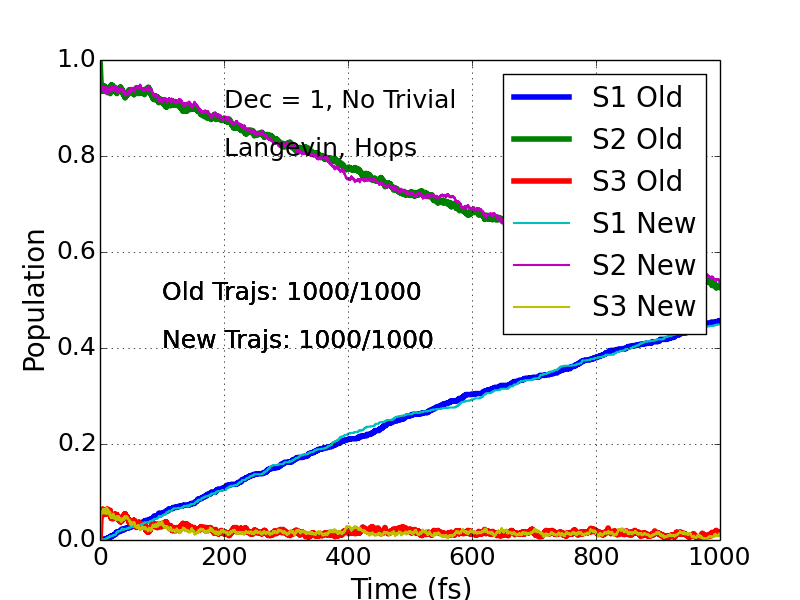
\includegraphics[scale=.35]{ppv_es_traj_decohere1_notrivial_langevin_hops_old_v_new.png}
            % 
        \end{subfigure}
	\hspace{3mm}
        \begin{subfigure}[h]{0.425\textwidth}  
            \centering 
            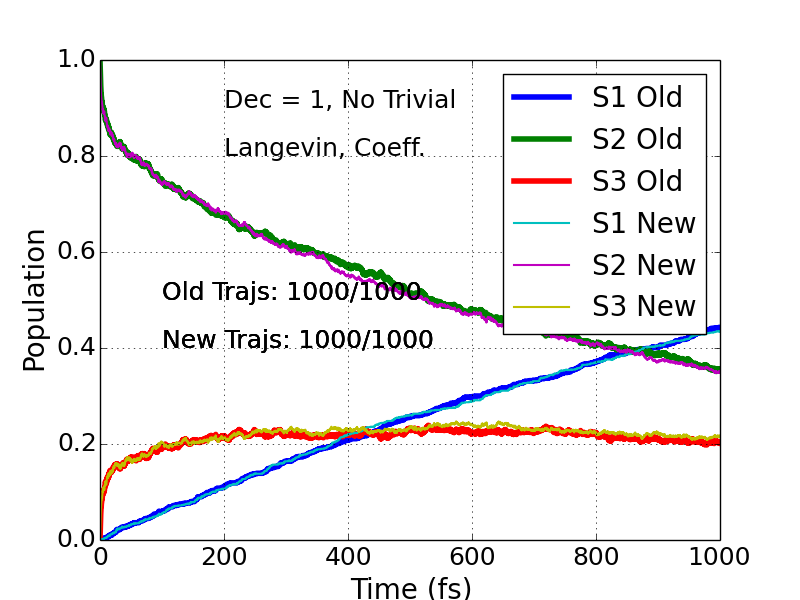
\includegraphics[scale=.35]{ppv_es_traj_decohere1_notrivial_langevin_coeff_old_v_new.png}
            %
        \end{subfigure}
	\begin{subfigure}[h]{0.425\textwidth}  
            \centering 
            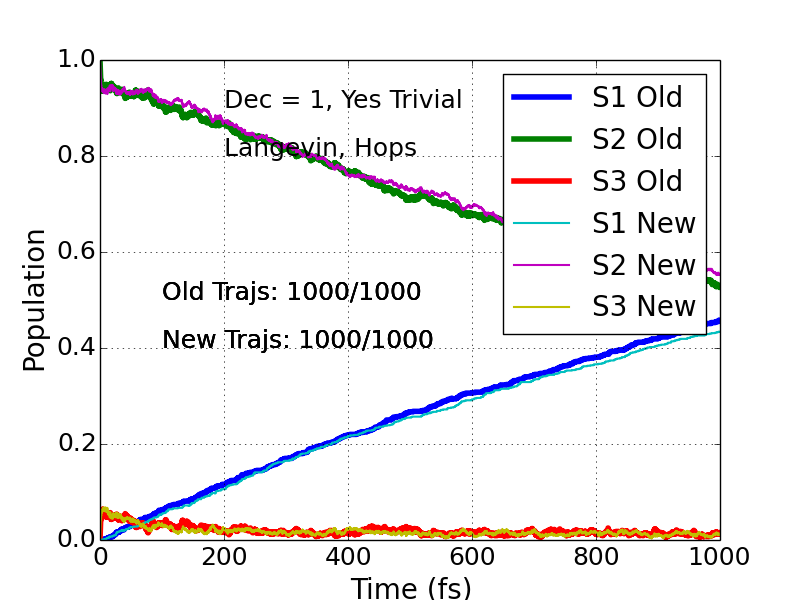
\includegraphics[scale=.35]{ppv_es_traj_decohere1_yestrivial_langevin_hops_old_v_new.png}
            %
        \end{subfigure}
	\hspace{3mm}
        \begin{subfigure}[h]{0.425\textwidth}   
            \centering 
            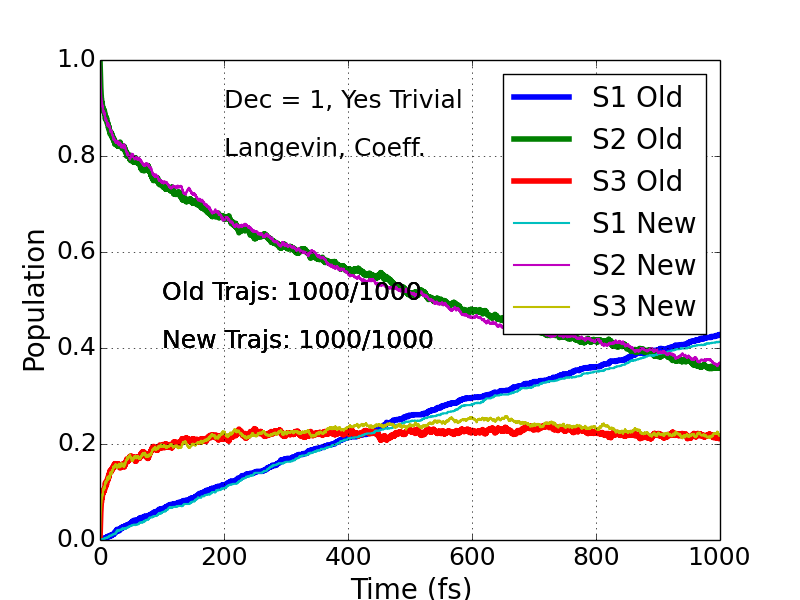
\includegraphics[scale=.35]{ppv_es_traj_decohere1_yestrivial_langevin_coeff_old_v_new.png}
            %
        \end{subfigure}
        \caption{\small Excited-state populations of a Poly(p-phenylene vinylene) (PPV3) molecule.  Each row is separate test, where 3 excited states were propagated.  Specification of the tests are labeled in the figures.  The {\textbf{left}} figures show populations from surface hopping, while the {\textbf{right}} figures show population from quantum coefficients.  Ensembles of 1000 trajectories were used.  For each trajectory, the system was initially excited on state $\ket{2}$.} 
\end{figure*}
\begin{figure*}[h]
        \centering
	\begin{subfigure}[h]{0.425\textwidth}  
            \centering 
            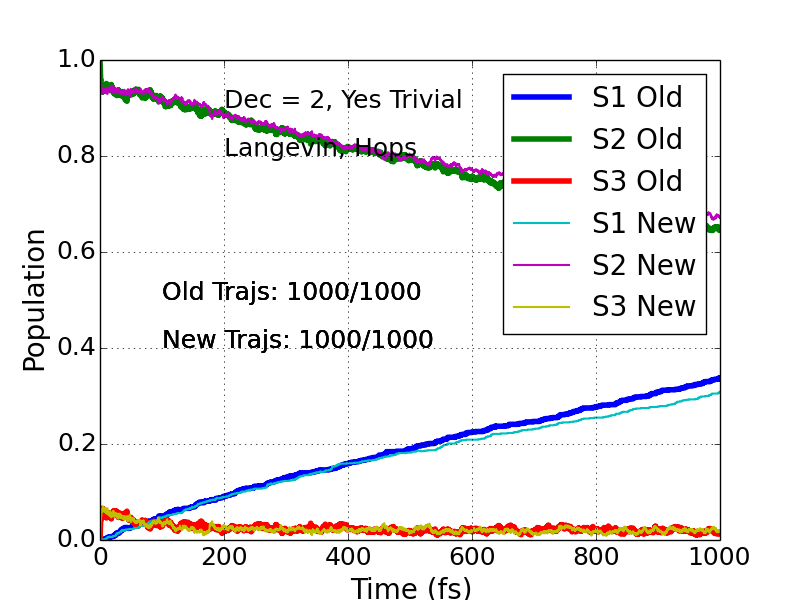
\includegraphics[scale=.35]{ppv_es_traj_decohere2_yestrivial_langevin_hops_old_v_new.png}
            %
        \end{subfigure}
	\hspace{3mm}
        \begin{subfigure}[h]{0.425\textwidth}   
            \centering 
            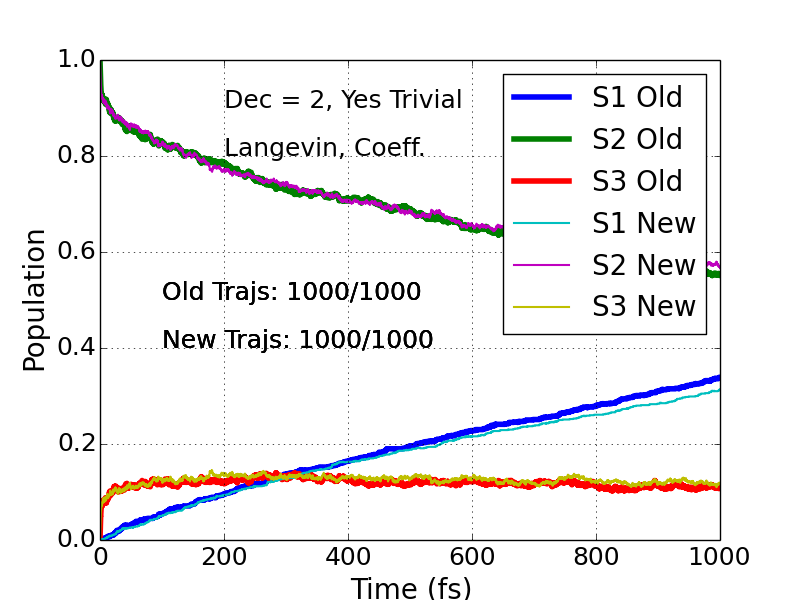
\includegraphics[scale=.35]{ppv_es_traj_decohere2_yestrivial_langevin_coeff_old_v_new.png}
            %
        \end{subfigure}
	\begin{subfigure}[h]{0.425\textwidth}  
            \centering 
            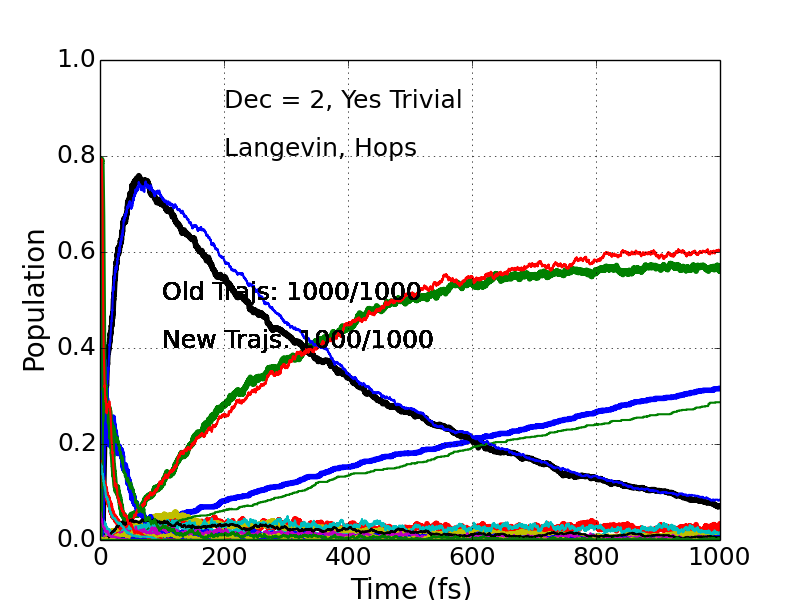
\includegraphics[scale=.35]{ppv_es_traj_decohere2_yestrivial_langevin_realistic_hops_old_v_new_opt.png}
            %
        \end{subfigure}
	\hspace{3mm}
        \begin{subfigure}[h]{0.425\textwidth}   
            \centering 
            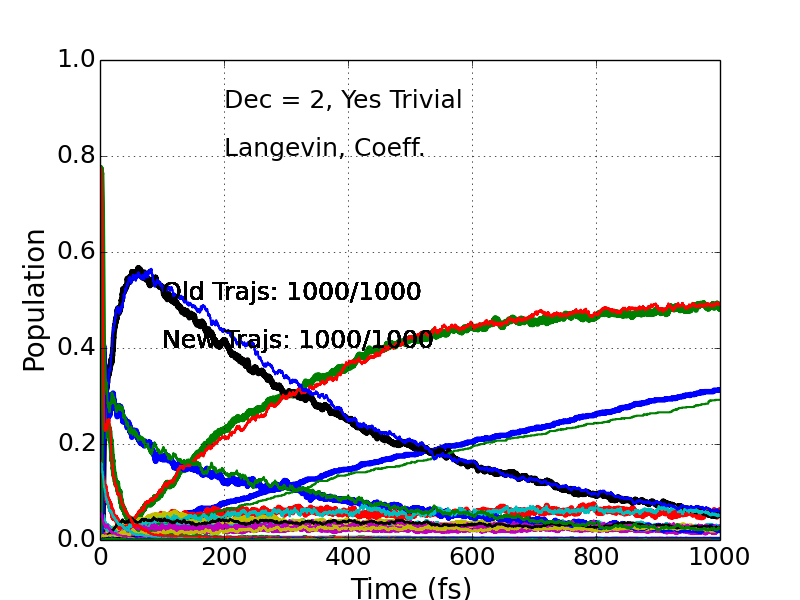
\includegraphics[scale=.35]
{ppv_es_traj_decohere2_yestrivial_langevin_realistic_coeff_old_v_new_opt.png}
            %
        \end{subfigure}
        \caption{\small Excited-state populations of a Poly(p-phenylene vinylene) (PPV3) molecule.  For {\textbf{top}} and {\textbf{bottom}} tests, 3 and 15 excited states were propagated, respectively.    Specification of the tests are labeled in the figures.  The {\textbf{left}} figures show populations from surface hopping, while the {\textbf{right}} figures show populations from quantum coefficients.  Ensembles of 1000 trajectories were used.  {\textbf{Top}}: All trajectories began on state $\ket{2}$.  {\textbf{Bottom}}: A distribution of initial excited states were chosen according to the system's theoretical optical absorption spectrum.} 
\end{figure*}
\begin{figure*}[h]
	\centering 
	\begin{subfigure}[h]{0.425\textwidth}  
            \centering 
	    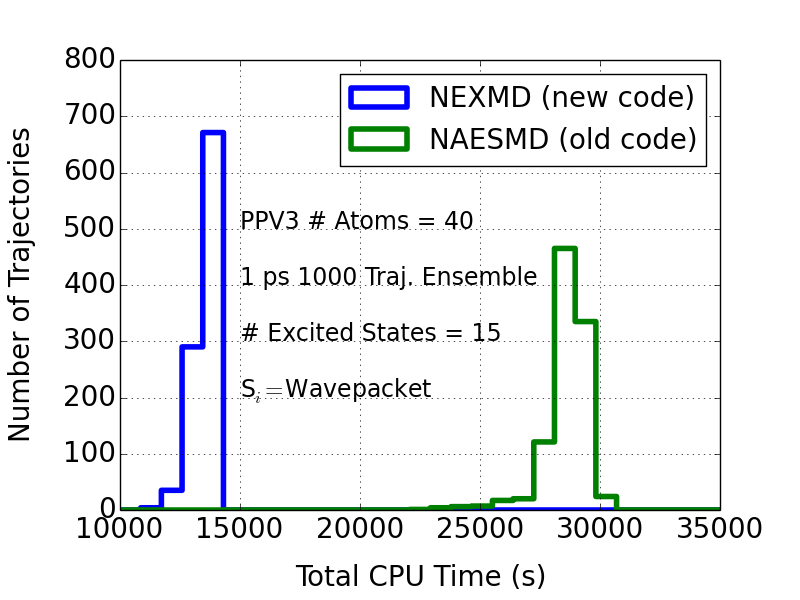
\includegraphics[scale=.35]{ppv_es_traj_decohere2_yestrivial_langevin_realistic_timings_hist.png}
            %
        \end{subfigure}
	\hspace{3mm}
        \begin{subfigure}[h]{0.425\textwidth}   
            \centering 
            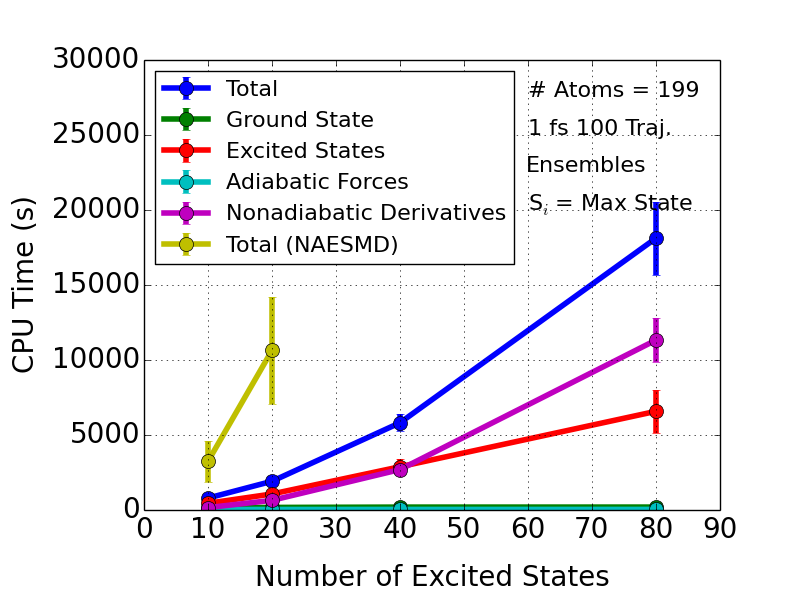
\includegraphics[scale=.35]
{timing_states_benchmark.png}
            %
        \end{subfigure}
        \begin{subfigure}[h]{0.425\textwidth}   
            \centering 
            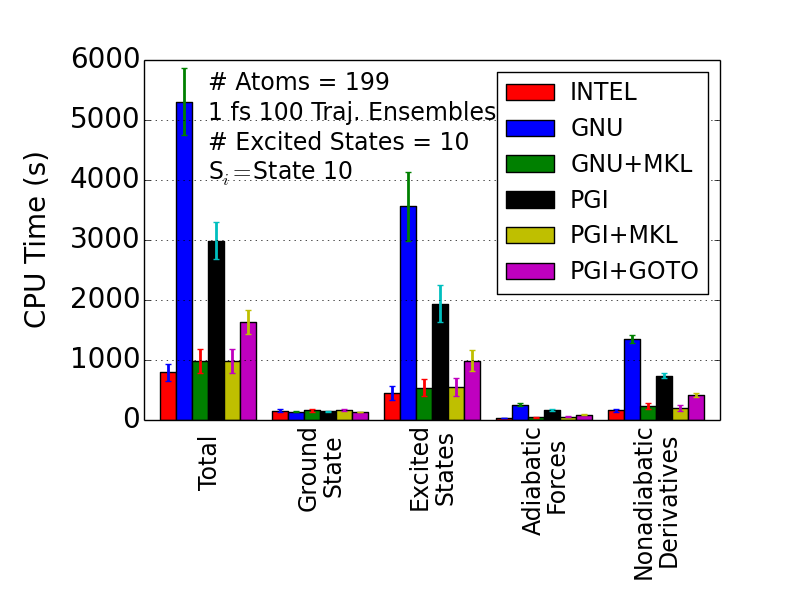
\includegraphics[scale=.35]
{timing_compiler_benchmark.png}
            %
        \end{subfigure}
        \begin{subfigure}[h]{0.425\textwidth}   
            \centering 
            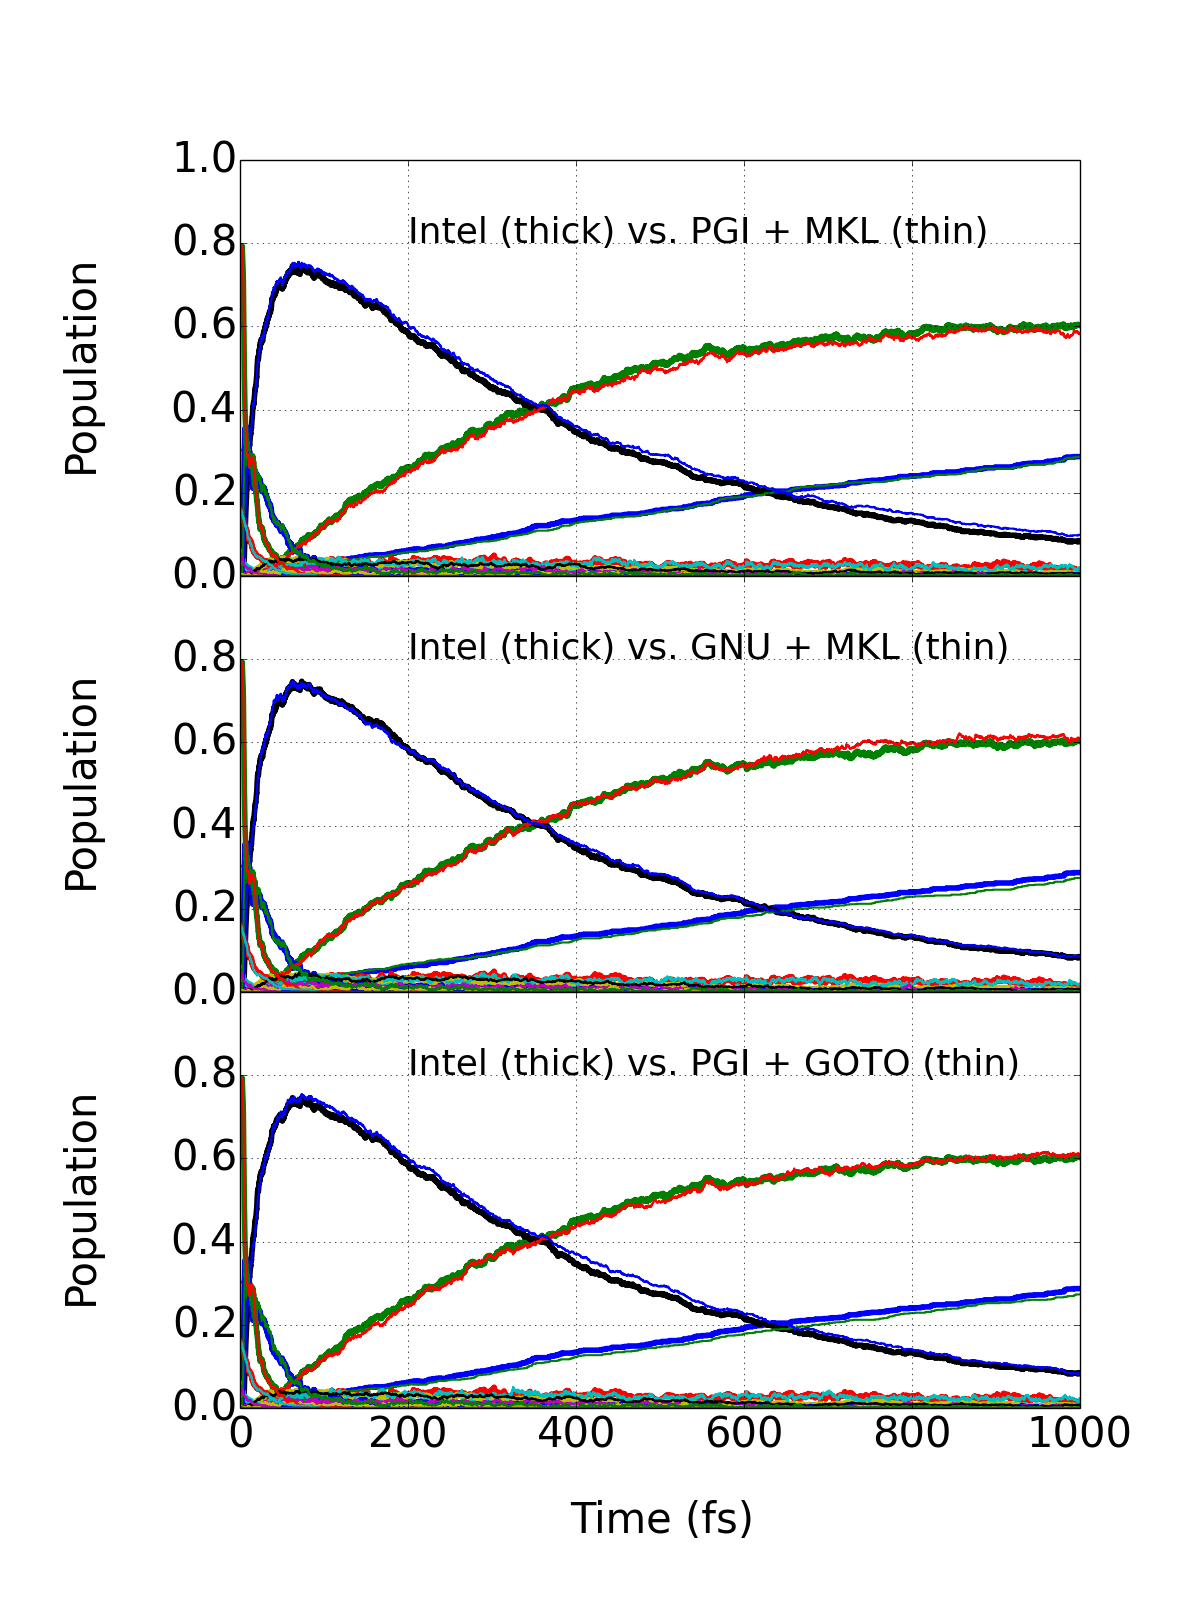
\includegraphics[scale=.25]
{population_compilers.png}
            %
        \end{subfigure}
	\caption{\small {\textbf{Upper Left}}: Total CPU time histogrammed over all trajectories used in the 1000-trajectory ensembles simulating the non-adiabatic dynamics of the Poly(p-phenylene vinylene) (PPV3) molecule with old and new codes. {\textbf{Upper Right}}: New code (NEXMD) timing performance as a function of the number of excited states propagated using a $\sim200$ atom system.  The mean and error (standard deviation) in CPU time of the 100-trajectory ensembles are shown.  Results of four separate simulations using 10, 20, 40, and 80 excited states are shown.  All trajectories began in the highest excited state.  Trajectories are 1 fs in length, with 0.10 fs classical step and 4 quantum steps per classical step.  All typical non-adiabatic inputs were used.  {\textbf{Lower Left}}: New code (NEXMD) timing performance as a a function of different compilers using a $\sim200$ atom system.  The mean and error (standard deviation) in CPU time of 100-trajectory ensembles are shown.  A total of 10 excited states were propagated and all trajectories began in the 10$^{\text{th}}$ excited state.  All typical non-adiabatic inputs were used.  {\textbf{Lower Right}}: New Code (NEXMD) consistency performance test against several compilers using 1000-trajectory ensembles simulating the non-adiabatic dynamics of the Poly(p-phenylene vinylene) (PPV3) molecule.  Version used are: GCC 5.3.0, PGI 16.10, GOTO, goto2r1.13, MKL/11.4.1}
\end{figure*}

\end{appendix}

\end{document}
